% This template was originally by R. Jacob Vogelstein
% Updated on March 1, 2010 by Noah J. Cowan

\documentclass[12pt,letterpaper, oneside,final]{template/thesisClass}
\special{papersize=8.5in,11in}
\pdfpagewidth 8.5in
\pdfpageheight 11.0in
\makeatletter
\let\@currsize\normalsize
\makeatother
\usepackage{acronym}
\usepackage{cite}
\usepackage{amsmath,amsfonts}
\usepackage{graphicx}
\graphicspath{{./figs/}}
\usepackage{fixltx2e}
\usepackage{array}
% wrapfig is fragile: use sparingly
\usepackage{wrapfig}
%\usepackage{times}  % Use this for ugly fonts
\usepackage[dvipsnames]{xcolor}
\usepackage{fancyhdr}    % Use nice looking headers along with the required footer page numbers
\usepackage{ifthen}
\usepackage{lettrine}
\usepackage{multirow}
\usepackage{hyperref}
%\usepackage[document]{ragged2e}
\usepackage{caption}
\usepackage{epigraph}
\usepackage{setspace}
\usepackage{subfigure}

%\usepackage[hypertex]{hyperref}

%Define the header/footer style
\pagestyle{fancy}
\fancyhf{}

\setlength{\headheight}{15pt}
%\lhead{\leftmark}
\cfoot{\thepage}
\renewcommand{\headrulewidth}{0pt}
\fancypagestyle{plain}{% Redefine ``plain'' style for chapter boundaries
\fancyhf{} % clear all header and footer fields

\fancyfoot[C]{\thepage} % except the center
\renewcommand{\headrulewidth}{0pt}
\renewcommand{\footrulewidth}{0pt}}
%\renewcommand\chaptername{}
%\renewcommand\chaptermark{1}
\renewcommand{\chaptermark}[1]{\markboth{ }{}}
\newcommand{\HRule}{\rule{\linewidth}{0.5mm}} % New command to make the lines in the title page
\newcommand{\notes}[1]{\textcolor{black}{\textbf{#1}}}


%\tolerance=10000

%\makeglossary % enable the glossary

\begin{document}

\title{Force Feedback for Patient Side Manipulator of Da Vinci Research Kit}
\author{Anna Novoseltseva}
\degreemonth{May}
\degreeyear{2018}
\copyrightnotice

% add your chapters, best way is to have separate TeX files for each chapter
%% FRONTMATTER

\begin{frontmatter}

	% generate title
	\maketitle
	
	\pagebreak
	\vskip 2em
			 {Approved by:\par}
			 \vskip 1em
			 \vspace{10 mm}
			 \ssp\rule[-2pt]{8cm}{0.5pt}\par
			 {Prof. Gregory S. Fischer, Advisor\par}
			 {Worcester Polytechnic Institute\par}
	
			 \vskip 1em
			 \vspace{10 mm}
			 \ssp\rule[-2pt]{8cm}{0.5pt}\par
			 {Prof. Karen Troy, Committee Member\par}
			 {Worcester Polytechnic Institute\par}
	
			 \vskip 1em
			 \vspace{10 mm}
			 \ssp\rule[-2pt]{8cm}{0.5pt}\par
			 {Prof. Loris Fichera, Committee Member\par}
			 {Worcester Polytechnic Institute\par}
	
	\begin{abstract}
Teleoperated robotic surgical systems such as daVinci are widely used for laparoscopic surgeries. The currently available daVinci system does not provide haptic feedback. Prior research has shown that the addition of haptic feedback improves surgeons' performance during minimally invasive surgeries. Other authors have implemented haptic feedback in the daVinci robot by placing sensors on the surgical tools, using visual force estimation, and measuring proximal guide wire forces. However, they have faced issues with biocompatibility, time delay, low accuracy, and repeatability. In this work, two strain gauge force-sensing devices were created for the patient side manipulator of the daVinci surgical robot. These devices were designed to be easily added to the existing system. The device mounted on the cannula measures the X-Y components of the forces applied to the tool, and the device mounted on the sterile adapter measures the Z-component of the force. These devices are used for the real-time force feedback in the daVinci robot. The proposed system has high sensitivity and resolution, matches the required force measurement range, and has high signal-to-noise ratio, which implies high signal quality. However, the absolute errors of the currently built devices are high. % ($error_x = -0.075 \pm 0.427 N$, $error_y = 0.1 \pm  0.9 N$, $error_z = -0.005 \pm 0.952 N$)
This work demonstrates fast 3-DOF force measurements on the daVinci robot without any robot modifications. While the present system has significant systematic errors, these can be mitigated by altering the mechanical design to reduce hysteresis and improve the accuracy of the system.

	\end{abstract}
	
	\begin{acknowledgment}
	
I would first like to thank my thesis advisor Professor Gregory Fischer. The door to Prof. [Last name] office was always open whenever I ran into a trouble spot or had a question about my research or writing. He consistently allowed this paper to be my own work, but steered me in the right the direction whenever he thought I needed it.

I would also like to thank the experts who were involved in the validation survey for this research project: [List professional Titles, Name and Surnames of the experts who participated/contributed]. Without their passionate participation and input, the validation survey could not have been successfully conducted.

I would also like to acknowledge [title] [Name Surname] of the [School / Faculty name] at [University name] as the second reader of this thesis, and I am gratefully indebted to his/her for his/her very valuable comments on this thesis.

Finally, I must express my very profound gratitude to my parents and to my boyfriend for providing me with unfailing support and continuous encouragement throughout my years of study and through the process of researching and writing this thesis. This accomplishment would not have been possible without them. Thank you.
	
	\end{acknowledgment}
	
	% generate table of contents
	\tableofcontents
	
	% generate list of tables
	\listoftables
	
	% generate list of figures
	\listoffigures
	
	Disclaimer: certain materials are included under the fair use exemption of the U.S. Copyright Law and have been prepared according to the fair use guidelines and are restricted from further use.
	
	\pagebreak
	\section*{Acronyms}
	\begin{acronym}
	\acro{PSM}{Patient Side Manipulator}
	\acro{DOF}{Degrees of Freedom}
	\acro{QTC Pills} {Quantum Tunneling Composite Pills}
	\acro{RMS}{Root Mean Square}
	\acro{PCB}{Printed Circuit Board}
	\acro{ROS}{Robot Operating System}
	\acro{SD}{Standard Deviation}
	\acro{SNR}{Signal-to-noise Ratio}
	\acro{GF}{Gauge Factor}
	\acro{ADC}{Analog to Digital Converter}
	\acro{FFT}{Fast Fourier transform}
	\acro{RMSE}{Root Mean Square Error}
	\end{acronym}
	
	\end{frontmatter}
	
	
\chapter{Introduction}
\label{intro} % Always give a unique label


Common ground. Teleoperated da Vinci surgical system is a robot-assisted surgical system that enhances surgeons performance in minimally invasive surgeries by allowing highly precise translation of surgeon`s hand movements to the instrument's movements. 

Practical problem condition. The currently available da Vinci surgery system has a laparoscopic camera, providing visual feedback to guide doctors during surgery. However, the system does not have any kinesthetic or cutaneous feedback, known as haptics.\cite{_intuitive_2018} 

The costs of that condition. 
During open surgeries, doctors usually get haptic feedback directly or through the surgical tools. In minimally invasive surgeries interaction with patients via long shafts leads to lose some forces and tactile senses since they have to . In robotic surgery systems, surgeons have to manipulate robots indirectly, which leads to an elimination of any haptic feedback. \cite{okamura_haptic_2009} 

It is believed that the addition of haptic feedback in the da Vinci surgery robot will help to reduce the amount of surgical errors and intra-operative injuries, which will lead to faster post-surgery recovery time and decreased rate of unsuccessful surgeries. \cite{reiley_effects_2008, van_der_meijden_value_2009, okamura_haptic_2009}

Gist of your solution. There are many technical challenges to overcome in order to implement the haptic feedback in da Vinci robot. One of them is getting accurate force readings from the patient side manipulator (PSM). To address this issue, we are trying to create force-feedback device, that can be easily added to the existing surgery system.
\chapter{Background}
\label{back}

\section{Teleoperated Surgical Robots}
\label{sec:daVinci}
Recently robots have started to be extensively used for surgical procedures. It allows doctors to perform these procedures with high accuracy, repeatability, and reliability, which in turn results in reducing operation time, errors and post-operation injuries. Minimally invasive surgeries are beneficial for accurate procedures with minimal access to operated organs, e.g. neurosurgery, eye surgery, cardiac surgery, intravascular surgeries and etc.  Use of robots in minimally invasive procedures improves precision and reliability of operations \cite{tavakoli_haptics_2008}.

There are two types of devices used for surgeries, supporting and augmenting. 

Supporting devices perform secondary functions to support the surgeon.  Some of them used for positioning and stabilization purposes of cameras, endoscopic tools, ultrasound probes and etc. Others to increase device dexterity or autonomy (dexterous and autonomous endoscopes).

Augmenting devices are used to extend surgeon's ability in performing an operation. They can be divided into four categories. Hand-held tools are augmenting instruments that used for hand tremors reduction, for dexterity and navigation capability increase. Another type of augmenting devices is cooperatively-controlled tools, where the surgeon and the robot cooperatively manipulate the surgical device (e.g. ROBODOC system, Steady- Hand robot, LARS, the Neurobot, and the ACROBOT system). Teleoperated robots are a type of augmenting tools, where a surgeon (master) controls the movements of a surgical robot (slave) via a surgeon's console (e.g. the daVinci system, Sensei X, Senhance). And autonomous tools, which can perform some tasks (suturing and knot tying) autonomously \cite{tavakoli_haptics_2008}.

Use of teleoperated robots in surgeries can solve many of the conventional surgery problems in terms of more precise manipulation capability, ergonomics, dexterity, and haptic feedback capability for the surgeon. They enhance dexterity by an increase of instrument degrees of freedom, hand tremor compensation, and movements scaling that allows transformation of the control grips large movements into small motions inside the patient. 3-D view with depth perception gives surgeons ability to directly control a stable visual field with increased magnification and maneuverability. All of these enhances the surgeon's performance. However, robot-assisted surgeries are high cost, need large operational room space, do not have established efficacy, and have a need for tableside assistants. For these reasons ability of hospitals to use surgical robots is low, making their use for routine surgeries improbable \cite{tavakoli_haptics_2008}.

Today, many surgical robotic systems have been commercially developed and approved by the FDA, such as the daVinci surgical system (Intuitive Surgical, Inc., Sunnyvale, CA) (Figure \ref{fig:daVinci}), Sensei X robotic catheter system (Hansen Medical Inc., Mountain View, CA), FreeHand v1.2 (FreeHand 2010 Ltd., Cardiff, UK), Invendoscopy E200 system (Invendo Medical GmbH, Germany), Flex® robotic system (Medrobotics Corp., Raynham, MA), Senhance (TransEnterix, Morrisville, NC) (Figure \ref{fig:Senhance}), Auris robotic endoscopy system (ARES; Auris Surgical Robotics, Silicon Valley, CA, USA), The NeoGuide Endoscopy System (NeoGuide Endoscopy System Inc, Los Gatos, CA) \cite{lanfranco_robotic_2004,peters_review_2018}.

\begin{figure}[h]
	\begin{center}
	\includegraphics[width=100mm]{fig/background/daVinciRobotPic.jpg}
	\end{center}
	\vspace{-4mm}
	\caption[The daVinci Xi Surgical System]
	{The daVinci Xi Surgical System}
	\label{fig:daVinci}
	\vspace{-2mm}
\end{figure}

There is also a number of NON-FDA-approved platforms that currently under development or going through clinical trials. For example, MiroSurge (RMC, DLR, German Aerospace Center, Oberpfaffenhofen-Weßling), The ViaCath system (BIOTRONIK, Berlin, Germany), SPORT™ surgical system (Titan Medical Inc., Toronto, Ontario), The SurgiBot™ (TransEnterix, Morrisville, NC), The Versius Robotic System (Cambridge Medical Robotics Ltd., Cambridge, UK), MASTER (Nanyang Technological University and National University Health System), Verb Surgical (Verb Surgical Inc., J \& J/Alphabet, Mountain View, CA, USA), Miniature in vivo robot (MIVR) (MIVR, Virtual Incision, CAST, University of Nebraska Medical Center, Omaha, Nebraska, USA), the Einstein surgical robot (Medtronic, Minneapolis, MN) \cite{peters_review_2018}.

\begin{figure}[h]
	\begin{center}
	\includegraphics[width=100mm]{fig/background/senhance.jpg}
	\end{center}
	\vspace{-4mm}
	\caption[The Senhance Surgical System]
	{The Senhance Surgical System}
	\label{fig:Senhance}
	\vspace{-2mm}
\end{figure}

The daVinci® surgical system is one of the most commonly used robotic surgical systems. In 2015, over 3400 systems were in use around the world. More than 3 million surgeries were performed worldwide using daVinci system \cite{_intuitive_2018}. The system has been approved for various types of surgeries such as cardiac, colorectal, thoracic, urological and gynecologic. However, new systems are emerging on the market, providing features that are absent currently in the daVinci System. For example, the Flex Robotic System, which consists of the flexible endoscope for laparoendoscopic surgeries. This system is able to define a non-linear path to surgical target by advancing a flexible telescopic inner-outer mechanism with instruments inside it, whereas instruments in the daVinci system can follow only non-flexible straight path. Another example is the Senhance robotic platform, which was cleared by the FDA in 2017, that provides actual haptic force feedback, allowing the surgeon to feel forces generated at the instruments end. In addition, the system uses eye-tracking technology to move the camera at the point the surgeon is looking at, while the daVinci uses a footswitch panel to control the camera movement \cite{peters_review_2018}.

%Effectiveness of daVinci system in comparison to opened surgery and other systems \cite{yu_safety_2014}


\section{Importance of Haptic Feedback}
\label{sec:hapticFeedbackImportance}

Several studies \cite{lim_role_2015, alleblas_effects_2017, currie_role_2017} have shown that implementation of force feedback into teleoperated robotic systems can reduce root-mean-square (RMS) and peak values of contact forces, energy consumption, a time required for task completion and the surgical errors rate \cite{tavakoli_haptics_2008}. The current version of daVinci robot does not provide haptic feedback, an addition of one would be beneficial for both patients and surgeons.

The addition of visual (2.16 ± 1.67), direct (1.62 ± 0.86), or both visual and direct force
feedback (2.15 ± 1.08) resulted in lower mean maximum force applied to mitral valve tissue while
suturing compared with no force feedback (3.34 ± 1.93 N; P < 0.05).
Conclusions To achieve better control of interaction forces on cardiac tissue during robotics assisted
mitral valve annuloplasty suturing, force feedback may be required. \cite{currie_role_2017}

The experimental results reveal reductions in force error (39.1% and
40.9%) when using haptic feedback during 1N and 2N pulling tasks. Moreover,
survey analyses showthe effectiveness of the haptic feedback during teleoperation.
Conclusions The combined tactile and kinesthetic feedback of the master
device in robotic surgery improves the surgeon’s ability to control the interaction
force applied to the tissue. \cite{lim_role_2015}

As reported by Cundy et al. [7], the experience of the each
single surgeon may probably explain these results. In fact
the personal expertise seems to overcome the lack of a
feedback haptic sensor, thus making feedback sensors
introduction desirable only if technologically and economically
feasible.

Mention 


\begin{figure}[h]
	\begin{center}
	\includegraphics[width=100mm]{fig/background/importance_haptics.png}
	\end{center}
	\vspace{-4mm}
	\caption[The Senhance Surgical System]
	{The Senhance Surgical System}
	\label{fig:Senhance}
	\vspace{-2mm}
\end{figure}

\section{Current Approaches}
\label{sec:CurAppr}

In order to implement haptic feedback in the daVinci system, it is necessary to create force sensing method for surgical tools first. Current approaches of incorporating force feedback include placement of force sensors on surgical tools, change of instruments design and some sensorless methods.

\subsection{Sensor Placement on Instrument}
\begin{itemize}
\item In \cite{hong_design_2012}, Hong et al. suggested measuring pulling and grasping forces at the tip of the surgical instrument by mounting strain gauges on top and bottom surfaces of each of the two flexure hinges of the forceps (Figure \ref{fig:integr_sen}). RMS errors were close to 0.1 N. One of the disadvantages of this method is biocompatibility issue due to contact of sensors and wires with patient tissues, another is increased cost of each tool. Taking into account that each instrument has limited lifespan \cite{ho_health_2011}, it will lead to significant increase in surgery cost.

\begin{figure}[h]
	\begin{center}
	\includegraphics[width=80mm]{fig/background/Sensor_on_instrument.pdf}
	\end{center}
	\vspace{-4mm}
	\caption[Prototype of the 2-DOF Compliant Forceps]
	{Prototype of the 2-DOF Compliant Forceps \cite{hong_design_2012}}
	\label{fig:integr_sen}
	\vspace{-2mm}
\end{figure}

\item  Some researchers use optical methods for force evaluation. These methods are divided by different sensing principles they use: intensity modulation, wavelength modulation, and phase modulation \cite{su_fiber_optic_2017}. In the paper \cite{_micro_2004}, authors developed 3-axial force sensor that uses light intensity modulation principle. It is based on a flexible titanium structure, that deforms with applied forces (Figure \ref{fig:opt_sen}). These deformations are measured through reflective measurements with three optical fibers. The method shows measurement force range 0.01 N to 2.5 N with 0.01 N resolution. The disadvantage of this method is narrow force measurement range.

\begin{figure}[h]
	\begin{center}
	\includegraphics[width=80mm]{fig/background/optic_meth.png}
	\end{center}
	\vspace{-4mm}
	\caption[Optical Force Sensor]
	{Optical Force Sensor \cite{_micro_2004}}
	\label{fig:opt_sen}
	\vspace{-2mm}
\end{figure}

\end{itemize}

\subsection{New Instrument Designs}
\begin{figure}[h]
	\begin{center}
	\includegraphics[width=100mm]{fig/background/new_instr_des.pdf}
	\end{center}
	\vspace{-4mm}
	\caption[Force-Sensing Surgical Tool]
	{ Force-Sensing Surgical Tool \cite{schwalb_forcesensing_2017}}
	\label{fig:force_sen_tool}
	\vspace{-2mm}
\end{figure}

Making new surgical instrument with implemented force sensors is another way to achieve force feedback \cite{schwalb_forcesensing_2017}. Authors developed the new force-sensing surgical tool, that uses a proximally located force/torque sensor (Figure \ref{fig:force_sen_tool}). This allows avoiding miniaturization and sterilization issues. The method has high sensing accuracy with errors less than 0.09 N. The outer diameter of the developed tool is 12 mm. This method as well requires an increase in the tool cost, leading to higher surgery expenses.

\subsection{Sensorless Methods}

All sensorless estimation methods avoid drawbacks associated with biocompatibility and integration issues. There are 2 methods: vision-based force feedback and motor currents measurement method.

\begin{itemize}
\item Some researchers proposed to use vision-based solution with supervised learning to estimate the applied forces. After extraction of the motion geometry of the object surface, they use a deep network to learn the relationship between the extracted visual information and the applied force. The evaluated average root-mean-square error of the method is 0.02 N.  The disadvantage of this methods is the necessity to know object’s material properties, and some materials such as bones would not visually deform. Additionally, the method has significant time delays due to computation time and is not suitable for real-time force feedback \cite{aviles_towards_2017}. 

\begin{figure}[h]
	\begin{center}
	\includegraphics[width=140mm]{fig/background/vision_based.png}
	\end{center}
	\vspace{-4mm}
	\caption[Flowchart of Vision-Based Force Estimation Approach]
	{Flowchart of Vision-Based Force Estimation Approach \cite{aviles_towards_2017}}
	\label{fig:visual_appr}
	\vspace{-2mm}
\end{figure}

\item In the papers \cite{sang_hongqiang_external_2017, yoon_design_2015}, authors estimate external forces using dynamics models and motor currents from the robot. They linearly parameterized PSM dynamics model and used it to derive forces values. As a result, they implemented sensorless force estimation method and they concluded that it was feasible. Even though, the proposed method does not show sufficient repeatability and accuracy.
\end{itemize}

\section{Force Sensing Technologies}
\label{sec:ForceSensors}

For the force sensing depending on their operating principle following types of sensors can be used: piezoelectric, strain-gauges, quantum tunneling composite pills (QTC Pills) or optical sensors \cite{SGandP1}.

\begin{itemize}
\item Piezoelectric sensors consist of two crystal disks with an electrode foil in between. When force is applied, an electric charge, proportional to the applied force, is obtained and can be measured. Piezoelectric sensors show small deformation when force is applied, this results in a high resonance frequency. Also, piezoelectric sensors due to their principle of operation have significant linearity error and drift \cite{SGandP2}.

\item QTC Pills are flexible polymers, that have exceptional electrical properties. They are made of a nonconducting material that contains small nickel particles.  In the resting state, it acts as an insulator, because metal particles are too far from each other. But when it is compressed, its conductivity increases and current can pass through it \cite{azaman_characteristic_2016}. QTC Pills are very sensitive and can work in wide ranged o forces. However, they have an exponential relationship between force and resistance, they are temperature sensitive and depend on charge application time. Meaning they have low accuracy and not suitable for dynamic force measurements \cite{_quantum_2010}.

\item In the strain gauge based force transducers the force causes deformation and subsequent linear change in resistance. Strain gauges are usually connected to a Wheatstone bridge circuit, where the output voltage is proportional to the applied force. Strain gauge based transducers provide small individual errors (200 ppm), show no drift, and are therefore appropriate for long-term monitoring tasks. However, they are relatively big, temperature dependent, and have a lower resonance frequency in comparison to piezoelectric sensors \cite{SGandP1,SGandP2}.

\item Optical retro-reflective sensors can be used for the force measurements. Emitter and receiver of these sensors are located at the same host. The light from the emitter goes through optical fibers reaches reflector and the reflected light goes back to the receiver. An interruption of the light beam due to bending can initiate a change of the signal output. Optical sensors are rarely used for force sensing applications because measurement range and sensing accuracy of such sensors are limited \cite{su_fiber_optic_2017}.
\end{itemize}

On the basis of the above mentioned, piezoelectric sensors are preferable for dynamic measurements of small forces while strain gauge sensors are better when large forces are measured. In this study, strain gauges were used since they show better accuracy and long-term stability \cite{SGandP1,SGandP2}.

\section{Contributions}
\label{sec:MyAppr}
Force sensing devices for measuring forces in X-Y direction and one for Z-direction measurement were created. They allow getting force readings from the daVinci tools of the PSM.  These devices can be easily added to the existing daVinci system. Since we have to add created device on each robot arm only, it is cheaper than placement of sensors on each separate surgical tool.  Moreover, created devices allow getting force data faster than through visual data processing method. And it has a chance to show better precision than motor current method.

\chapter{Methods and Results}
\label{methods} % Always give a unique label
%use
% to alter or adjust the chapter heading in the running head

\section{Force Measurement}
\label{sec:sysArch}

\begin{figure}[h]
	\begin{center}
		\includegraphics[width=100mm]{fig/methods/the_device.png}
	\end{center}
	\vspace{-4mm}
	\caption[Developed Force Measuring System Attached to the PSM]
	{Developed Force Measuring System Attached to the PSM}
	\label{fig:PSM_with_FF}
	\vspace{-2mm}
\end{figure}

Block diagram of the created system for 3-DOF force measurement is shown on figure \ref{fig:BlockDiag}. Forces that applied on the end of surgical tool are measured using strain gauges, which change their resistance with force. Using created printed circuit boards (PCBs), this resistance changes are measured and published within ROS. At the same time we measure current joint position of the tool, which is needed for the force calibration. The position data and data from PCBs are used to find values of the force in X,Y,Z directions.

\begin{figure}[h]
	\begin{center}
		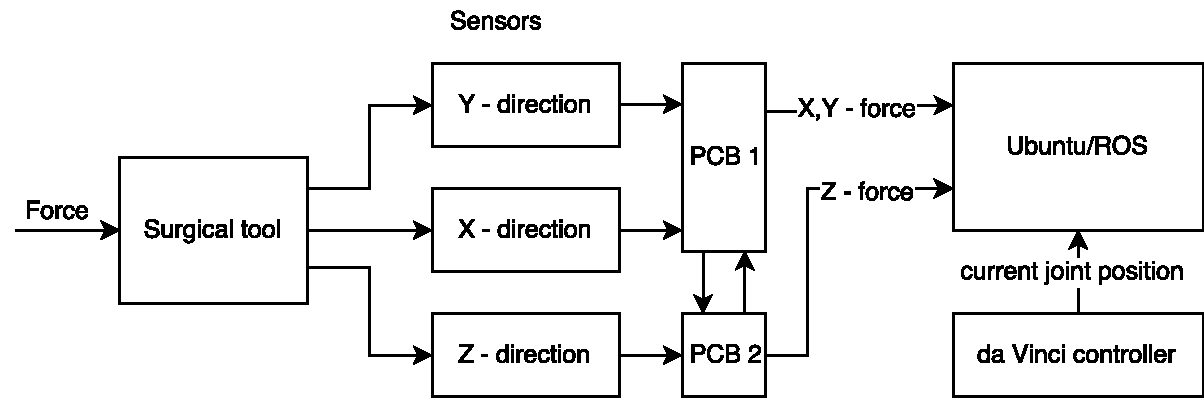
\includegraphics[width=140mm]{fig/methods/dbd2.pdf}
	\end{center}
	\vspace{-4mm}
	\caption[Block Diagram]
	{Block Diagram}
	\label{fig:BlockDiag}
	\vspace{-2mm}
\end{figure}

\section{Sensor Placement Optimization}
\label{sec:SimMod}
A finite element analysis was done in Solidworks to assess better placement of the strain gauges on the created device. In order to run finite element analysis material properties, such as elastic modulus, poisson`s ratio, and density are necessary to know. Sleeve material is aluminum 6061, that has elastic modulus 68.9 GPa, poisson`s ratio 0.33, and density 2700 kg/m\textsuperscript{3} \cite{aluminum_properties}. Since the shaft and cannula materials are unknown, in order to run finite element analysis their elasticity modulus and density were found experimentally.
	
	\subsection{Elastic Modulus Measurements}
	\label{sec:ElasMod}
	Elastic Modulus of the shaft and the cannula were found experimentally (Figure \ref{fig:ElasModSet}). One end of the observing sample (shaft/cannula) was fixed and the force was applied on the other end. We used weights 250g for the shaft and 555g for the cannula to apply forces. The deformation caused by forces was detected with dial indicator. Experiment was done 5 times, average displacement value was used to calculate elastic modulus. Results are shown in Table \ref{tab:elasMod}.
	
\begin{figure}[h]
	\begin{center}
		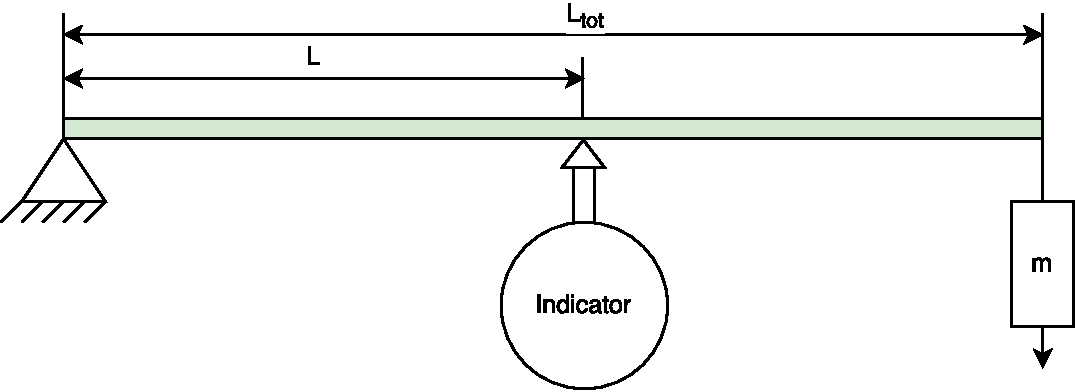
\includegraphics[width=120mm]{fig/methods/el_mod_set.pdf}
	\end{center}
	\vspace{-4mm}
	\caption[Setup to Measure Elastic Modulus]
	{Setup to Measure Elastic Modulus}
	\label{fig:ElasModSet}
	\vspace{-2mm}
\end{figure}

\begin{table}
\caption {Elasticity Modulus Measurement Data} \label{tab:elasMod} 
\begin{tabular}{ | c | c | c | c | c | c | c | c | } 
\hline
Component & $d_o$, mm & $d_i$, mm & $I$, mm\textsuperscript{4} & $m$, g & $F$, N & $L$, mm & $L_{tot}$, mm \\ 
\hline
Shaft & 8.4 & 6 & $1.808 \cdot 10^{-10}$ & 250 & 3.25 & 276.2 & 366.8\\ 
\hline
Cannula & 10.54 & 8.75 & $3.181 \cdot 10^{-10}$ & 555 & 6.011 & 95.5 & 105.55 \\ 
\hline
\end{tabular}

\begin{tabular}{ | c | c | c | } 
\hline
Component & $\delta \pm SD$, mm & $E \pm SD$, GPa \\ 
\hline
Shaft & $2.856 \pm 0.123$ & $44.31 \pm 1.86$ \\ 
\hline
Cannula & $0.086 \pm 0.004$ & $63.92 \pm 2.97$ \\ 
\hline
\end{tabular}
\end{table}

Elastic Modulus was found using following equation:

\begin{equation}
E = \frac{FL^3}{3 \delta I} 
\end{equation}

where $F$ - force, $L$ - length from the fixed point to indicator, $I$ - area moment of inertia, $\delta$ - displacement.

Area moment of Inertia: 
\begin{equation}
I = \frac{\pi (d_o^4 - d_i^4)}{64}
\end{equation}

where $d_o$ - cylinder outside diameter, $d_i$- cylinder inside diameter.

Force acting on indicator:
\begin{equation}
F = \frac{L_{tot}}{L}mg
\end{equation}

where $L_{tot}$ - total length of the object, $m$ - mass of the weight, $g$ - gravitational constant.

Experimentally found mean value of elastic modulus of the shaft is equal to 44.31 GPa with standard deviation (SD) 1.86 GPa, elastic modulus of the cannula is 63.92 GPa with SD 2.97 GPa.

	\subsection{Density Measurements}
	\label{sec:DenMeas}
Density was found using following equation:

\begin{equation}
p=\frac{m}{V}
\end{equation}

where $m$ - mass, $V$ - volume.

Weight was measured using mechanical scale. Volume of the shaft was found by following equation: $V =  \pi h(r_o^2-r_i^2) = 4.36 \cdot 10^{-5} m^3$. Volume of the cannula was found using water displacement method. Shaft material density is 473 kg/m\textsuperscript{3}, cannula material density is 55238 kg/m\textsuperscript{3}.

\subsection{Simulation Results}
\label{sec:FEAres}
The mounting location of the active strain gauges should be under the greatest amount of strain. From the Figure \ref{fig:XYdev}, it can be seen that strain gauges for X-Y direction device should be mounted on the area shown green, that corresponds to strain value approximately equal to $1.5 \cdot 10^{-4}$. Passive strain gauges, that will be used only for temperature compensation, will be placed on the blue area perpendicular to the active strain gauges.

\begin{figure}[h]
	\begin{center}
		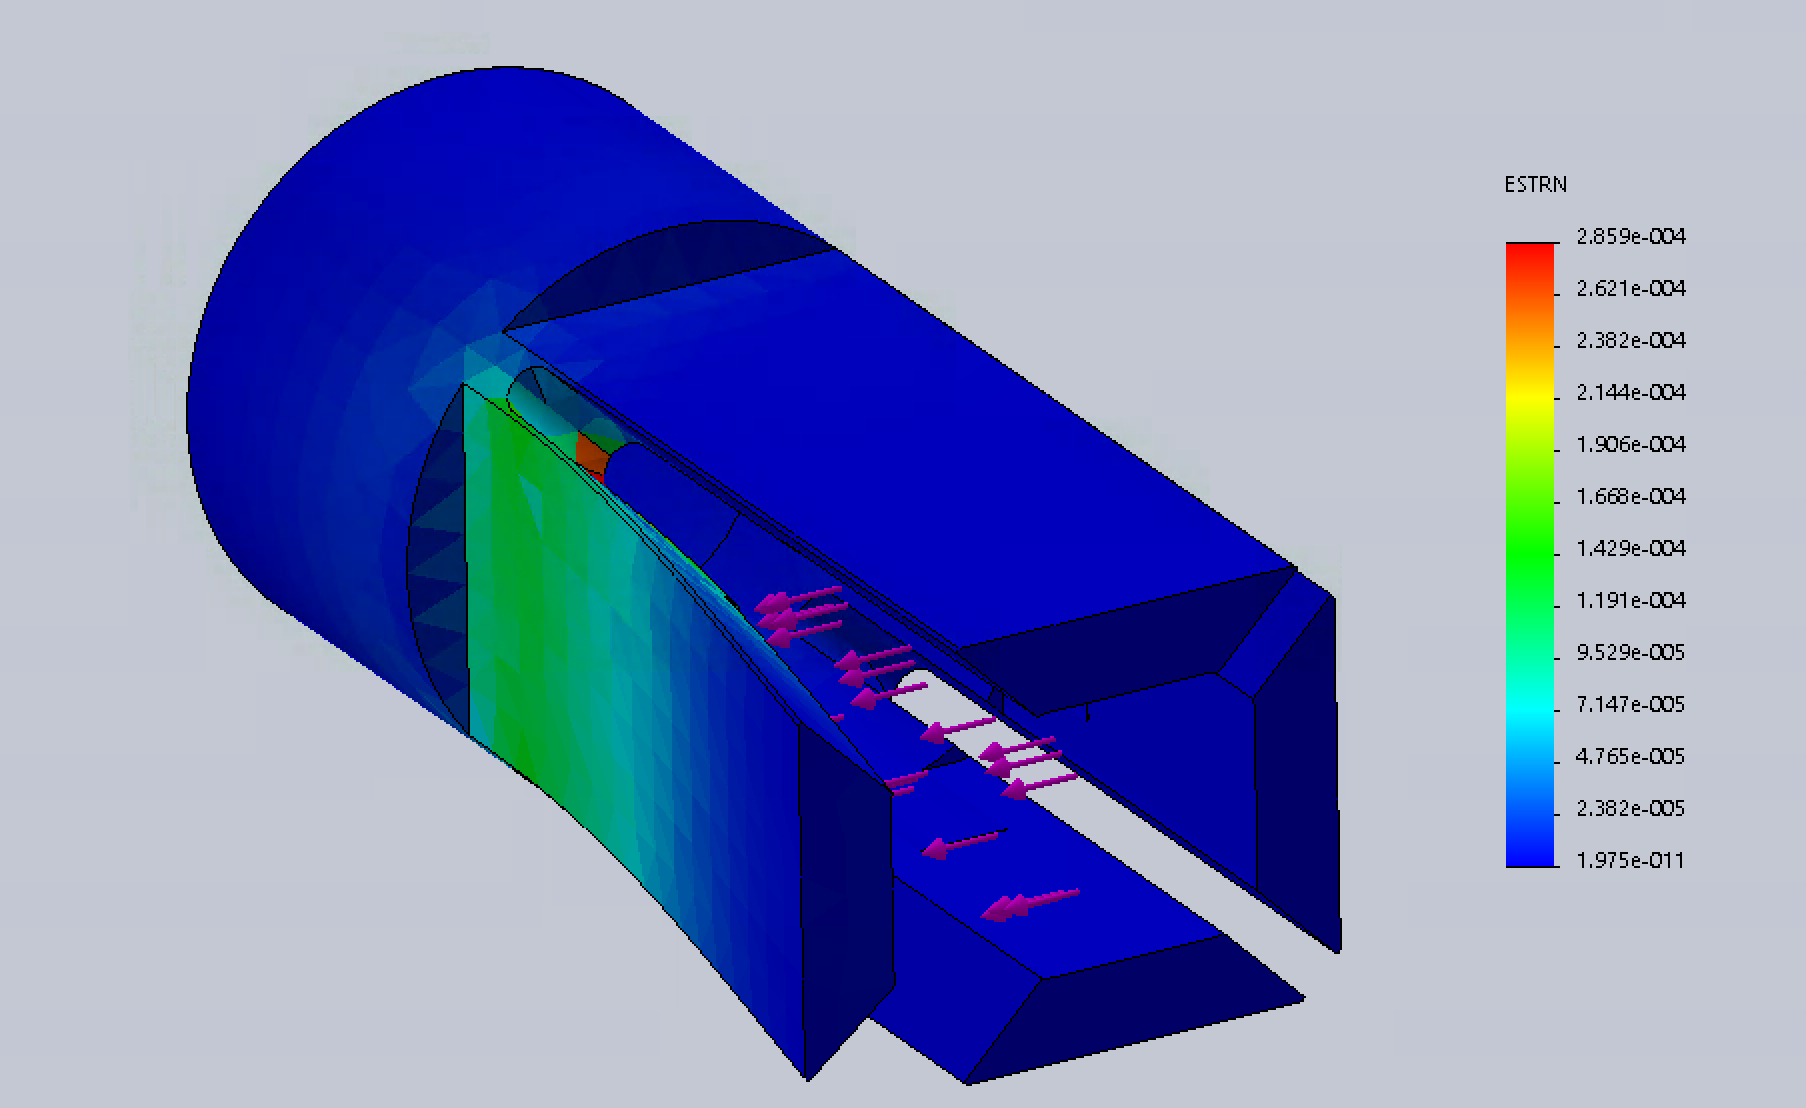
\includegraphics[width=100mm]{fig/methods/old_sleeve.png}
	\end{center}
	\vspace{-4mm}
	\caption[X-Y device]
	{Strain in the Device to Measure Forces in X-Y Direction}
	\label{fig:XYdev}
	\vspace{-2mm}
\end{figure}


\begin{figure}[h]
	\begin{center}
		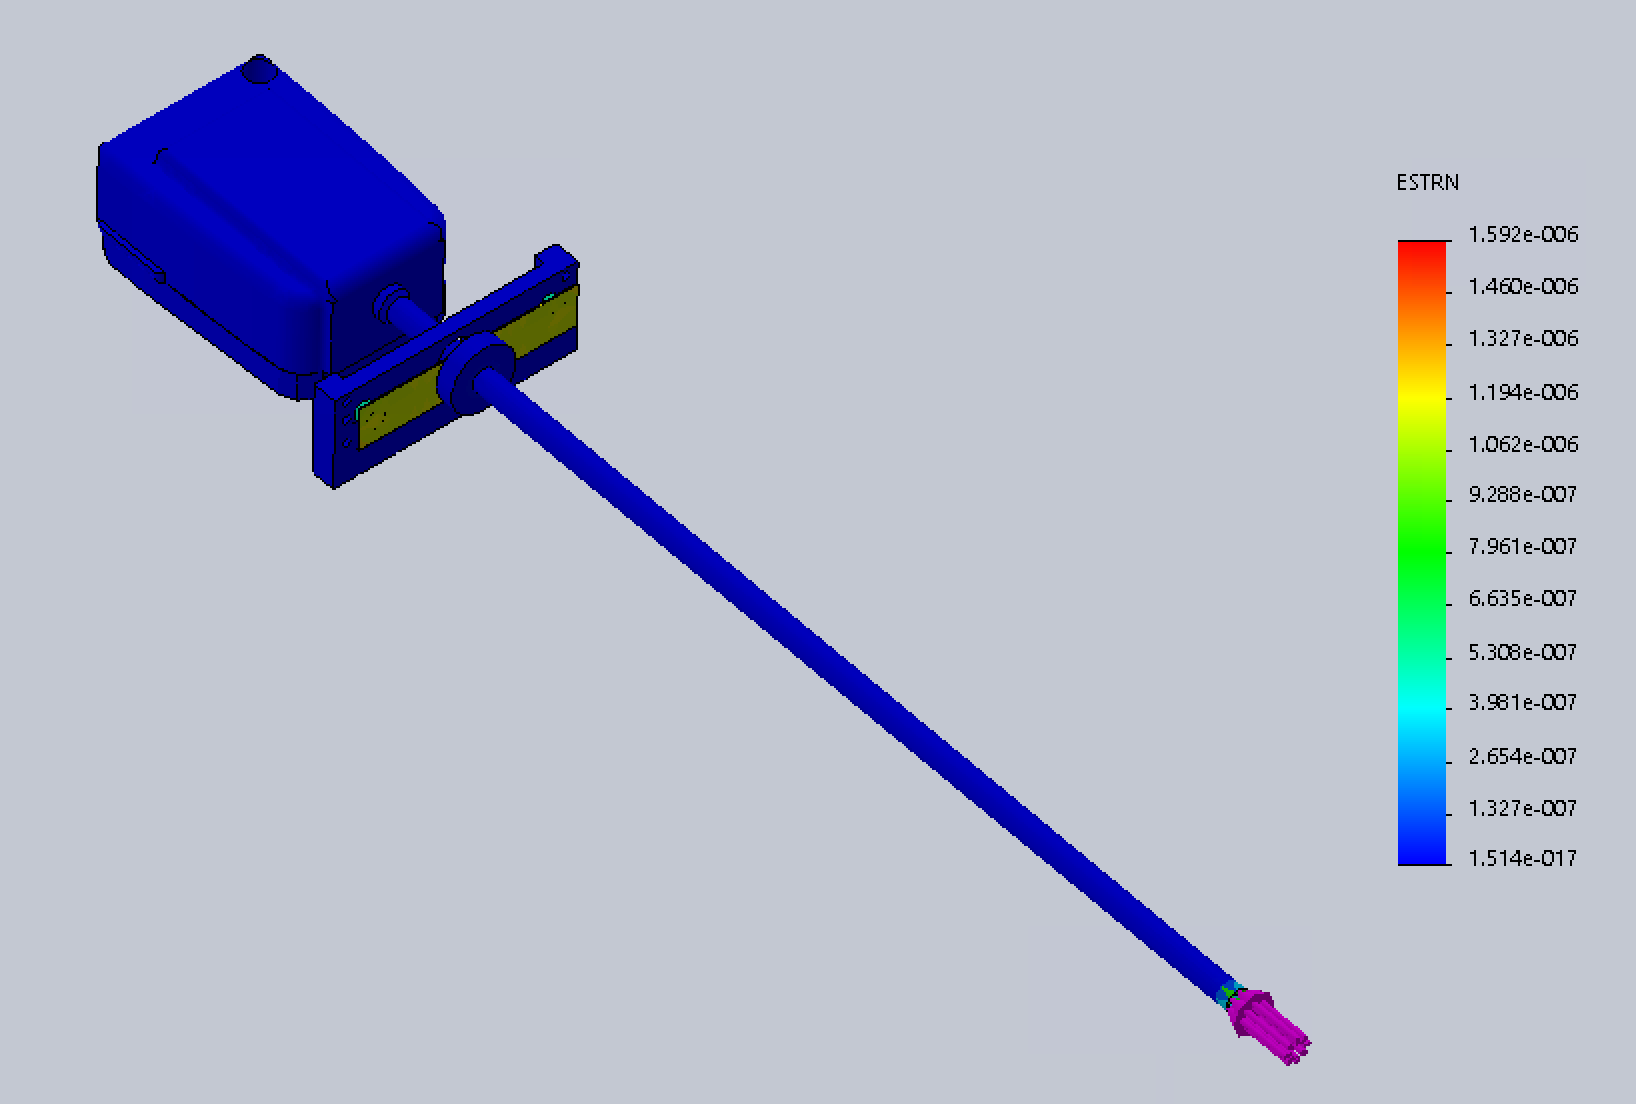
\includegraphics[width=100mm]{fig/methods/z_dir_sim.png}
	\end{center}
	\vspace{-4mm}
	\caption[Z device]
	{Strain in the Device to Measure Forces in Z Direction}
	\label{fig:Zdev}
	\vspace{-2mm}
\end{figure}

For Z-direction measurement forces (Figure \ref{fig:Zdev}), area shown with yellow-green color under the highest strain. On both sides and both ends of this plate strain gauges should be placed to form full bridge.

\begin{table}
\caption {Material Properties} \label{tab:matProp} 
\begin{center}
\begin{tabular}{ | c | c | c | c | c | c | c | c | } 
\hline
Component & Elastic Modulus, GPa & Density, kg/ m\textsuperscript{3} \\ 
\hline
Shaft & 44.31 & 473\\ 
\hline
Cannula & 63.92 & 55238 \\ 
\hline
Sleeve & 68.9 & 2700  \\ 
\hline
\end{tabular}
\end{center}
\end{table}

All material properties used for simulations are listed in Table \ref{tab:matProp}.

\section{Requirements for the Device}
	\label{sec:DevReq}
	From the literature review, following requirements for the device were outlined:
	
	Biocompatibility: Z-device is attached to sterile adapter and does not have to be biocompatible. X-Y device goes inside the patient, it means that it should be sterilized and created using biocompatible materials. Current version of the device is not biocompatible. We can achieve biocompatibilty by using Stainless Steel as a device material and biocompatible epoxy to cover strain gauges, also teflon coated wires should be used for all electrical connections.
	
	Force range: Some studies \cite{mack_interactive_2012, prasad_modular_2003, } have shown that force range applied during surgeries lies in range (0-11 N). The designed device measures forces in that range, and if the force goes beyond that range it can be used to trigger safety alert.
	
	Force sensitivity: The device should be sensitive enough with minimum detectable signal (MDS) at least 0.3 N and give accurate readings (error < 0.05 N) \cite{mack_interactive_2012}.
	
	Speed of force reading: Device is used for real-time haptic feedback, the minimum requirement for data acquisition speed is 1 kHz \cite{seungmoon_choi_effect_2004}.
	
	No restriction of motion range of the device: We were able to measure force in three directions independently from each other using separate wheatstone bridges for each direction. At the same time tool can rotate freely and change depth of insertion.	
	
	Linearity: Strain gauges have linear response with deformation. Our calibration results have shown linearity of the readings.

	Device modularity: Force-sensing devices were designed to fit daVinci cannula and sterile adapter and compensate tolerances by adjustment of set screws.
	
\section{Mechanical Design}
\label{sec:mechDes}

	\subsection{Strain Gauge}
	\label{sec:SGReq}
	According to the manual for strain gauge selection provided by Vishay Micro-Measurements, the strain gauge should have following parameters:
\begin{itemize}
  \item Single grid for unidirectional force measurements;
  \item Isoelastic (D alloy) that has higher gauge factor with E backing;
  \item Encapsulated with pre attached leads for easier placement;
  \item STC (self-temperature-compensation) - small temperature dependence;
\end{itemize}	
	
Maximum strain on the created device is $1.5 \cdot 10^{-4}$, in case of 10 N load with maximally opened shaft. From the literature, strain gauges length should be more than 5\% of maximum strain, hence, minimum length of the strain gauge should be 0.0075 mm. 

Gauge Factor (GF) for strain gauges usually is 2. According to the formula (\ref{eq:resistance}) strain gauge with resistance 120 $\Omega$ have maximum change in resistance equal to 0.036 $\Omega$, and 350  - 0.105 $\Omega$:

\begin{equation}\label{eq:resistance}
\Delta R=GF \cdot R \cdot \varepsilon
\end{equation}

where $GF$ - gauge factor, $R$ - resistance, $\varepsilon$- strain.

For the device strain gauges with resistance 350 $\Omega$, GF is 2, single grid, encapsulated with pre-attached leads were used.

	\subsection{Installation of Strain Gauges}
	\label{sec:instSG}

	Application of strain gauges was done following the manual provided by Vishay Micro-Measurements. \cite{StrGugeInst}.

	First the working surface (glass) and tweezers were cleaned with Neutralizer 5. 
	After that shaft surface preparation was started, using solvent degreaser GC-6 Isopropyl Alcohol. 
	A gauge layout was then applied with a 4H drafting pencil. The surface was then conditioned with Conditioner A and the extra liquid was wiped with gauze. 
	Finally, the surface was then neutralized with M-Prep Neutralizer 5A. \cite{StrGugeInst}

	The strain gauges were first placed on the glass and then transported using mylar tape onto the instrument surface. A thin layer of catalyst was applied on the strain gauge and given one minute to dry. Then adhesive M-BOND 200 was applied on the surface, pressure was applied on the tape for one minute, then two more minutes to let it dry before the tape was removed. Then leads soldering was done by application of pats, and soldering them with thin wires. \cite{youtube}

	The methodology of the strain gauge application more specifically described in \cite{StrGugeInst}.

	In compliance with the literature \cite{StrGugeInst} for application of the strain gauge on metals, the same materials and technique can be used. Therefore, the same method was used to apply strain gauges on different materials.

\subsection{X-Y direction}
\label{sec:xyDir}

XY-device consists of one sleeve and one set screw. We manufactured sleeve using Aluminum 6061 Alloy. %First, hole with diameter 9.5 mm should be drilled in the center using the lathe machine. Then on the milling machine all the side slots and inner square should be milled. On the same machine hole for the set screw should be drilled. After that set screw thread was tapped.%
The manufactured sleeve is placed on the cannula end and is fixed with a set screw on the top.

\begin{figure}[h]
	\begin{center}
		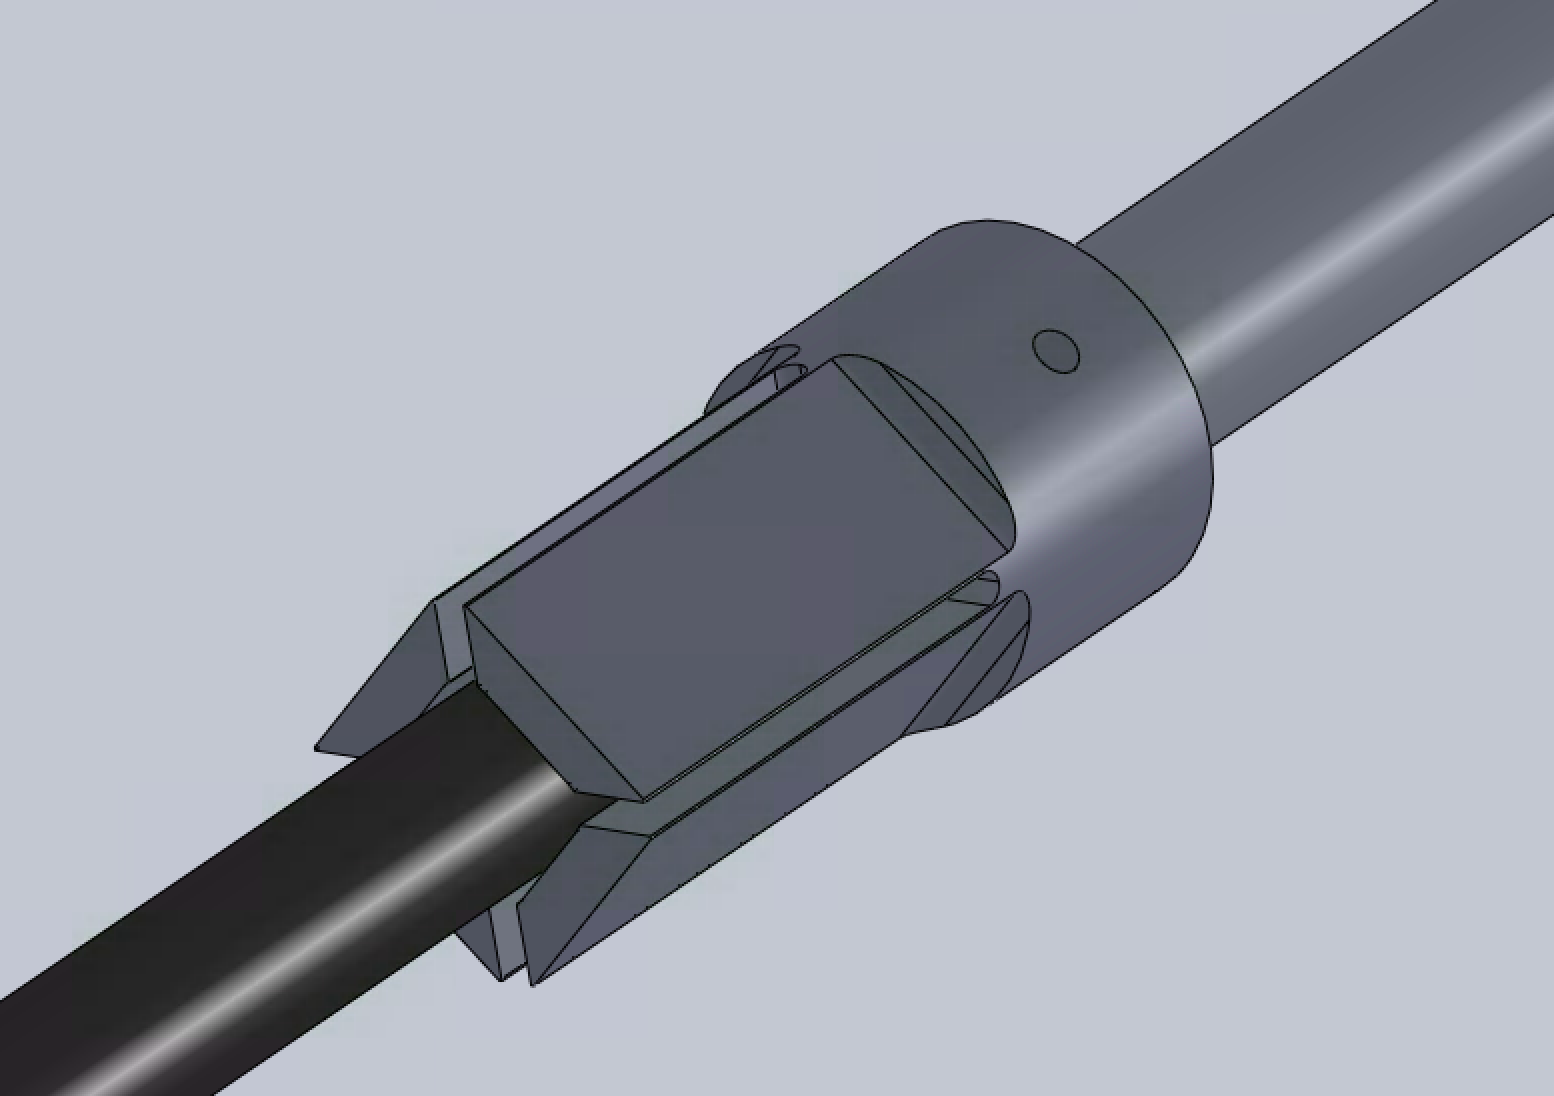
\includegraphics[width=80mm]{fig/methods/xy_dev_cl.png}
	\end{center}
	\vspace{-4mm}
	\caption[XY-direction force feedback sensor]
	{XY-direction Force Feedback Fensor}
	\label{fig:xy-direction}
	\vspace{-2mm}
\end{figure}

\begin{figure}[h]
	\begin{center}
		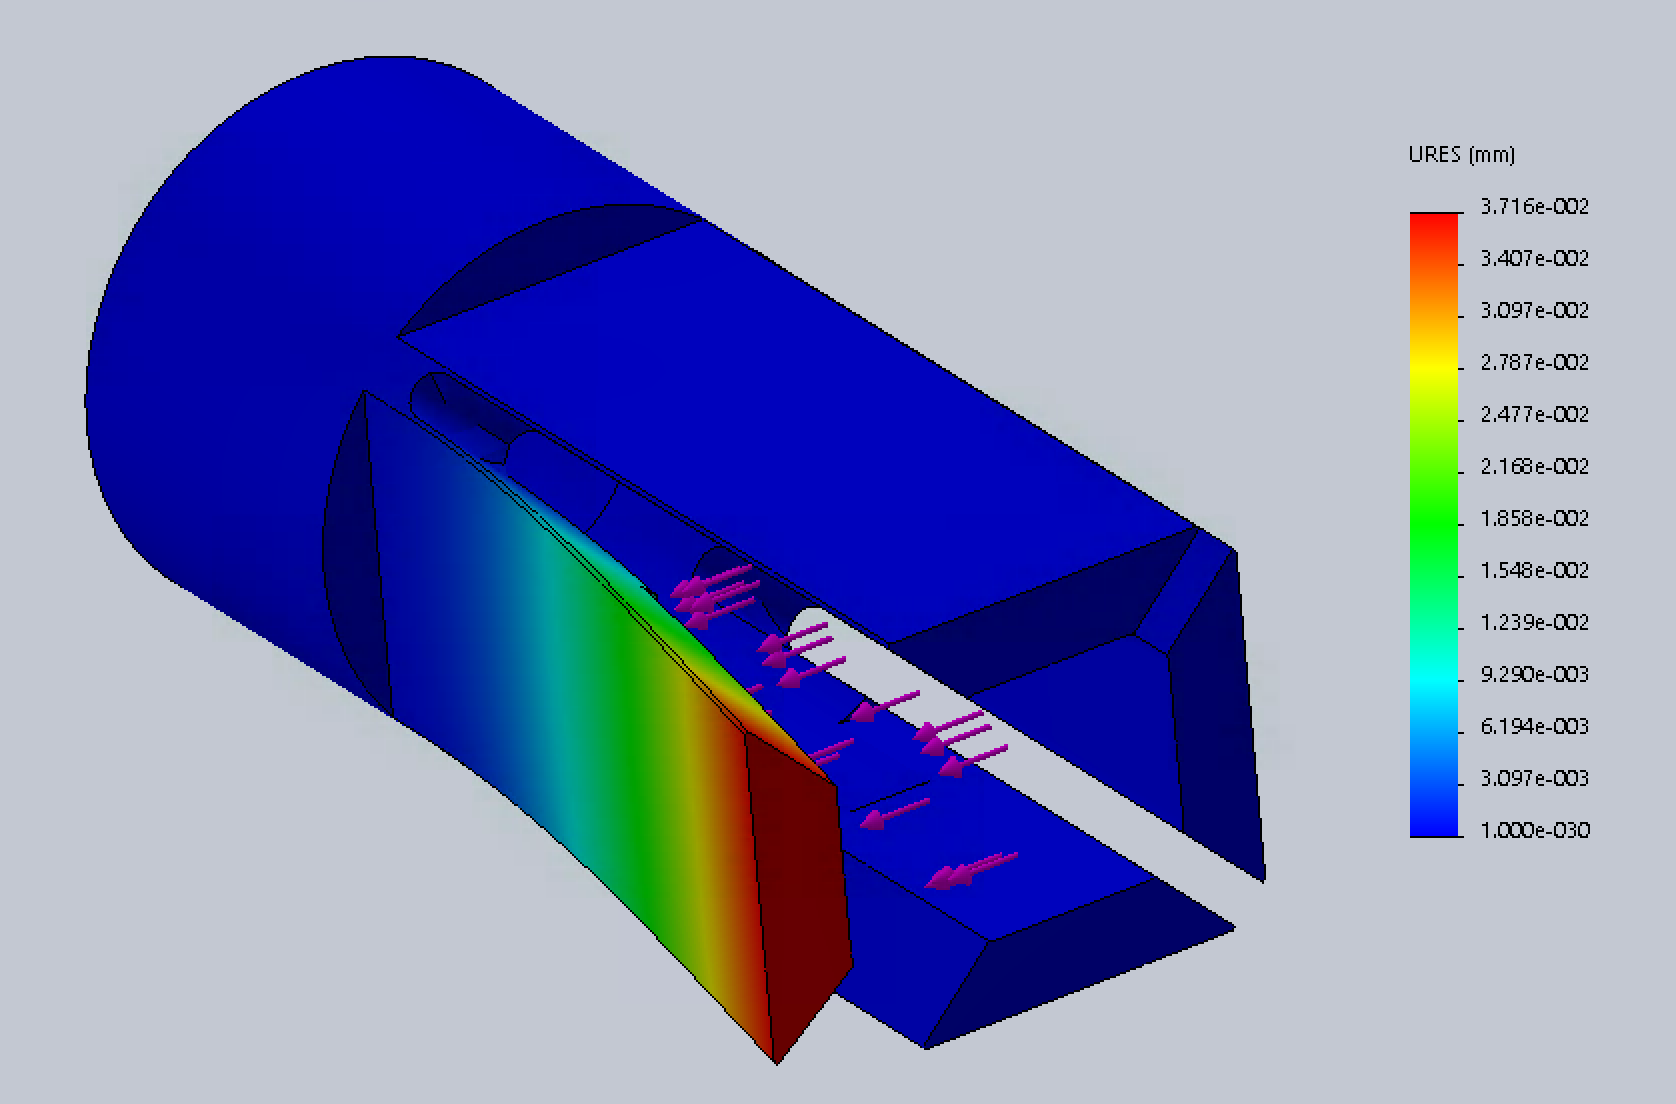
\includegraphics[width=80mm]{fig/methods/old_sleeve_displ.png}
	\end{center}
	\vspace{-4mm}
	\caption[XY-direction force feedback sensor]
	{Displacement of the XY Device}
	\label{fig:xy-displ}
	\vspace{-2mm}
\end{figure}

In order to get accurate readings maximum displacement of the sleeve sides should prevent shaft from hitting the cannula. It means that it should be less than $d=(d_{can_in} - d_{shaft_out})/2 = (8.75 - 8.4)/2 = 0.175$ mm. From the Solidworks simulation (Figure \ref{fig:xy-displ}), maximum displacement is 0.037 mm, which is in appropriate range.

\subsection{Z-direction}
\label{sec:zDir}

\begin{figure}[h]
	\begin{center}
		\includegraphics[width=80mm]{fig/methods/z_dir_design.png}
	\end{center}
	\vspace{-4mm}
	\caption[Z-direction force feedback sensor]
	{Z-direction Force Feedback Fensor}
	\label{fig:Z-direction}
	\vspace{-2mm}
\end{figure}

\begin{figure}[h]
	\begin{center}
		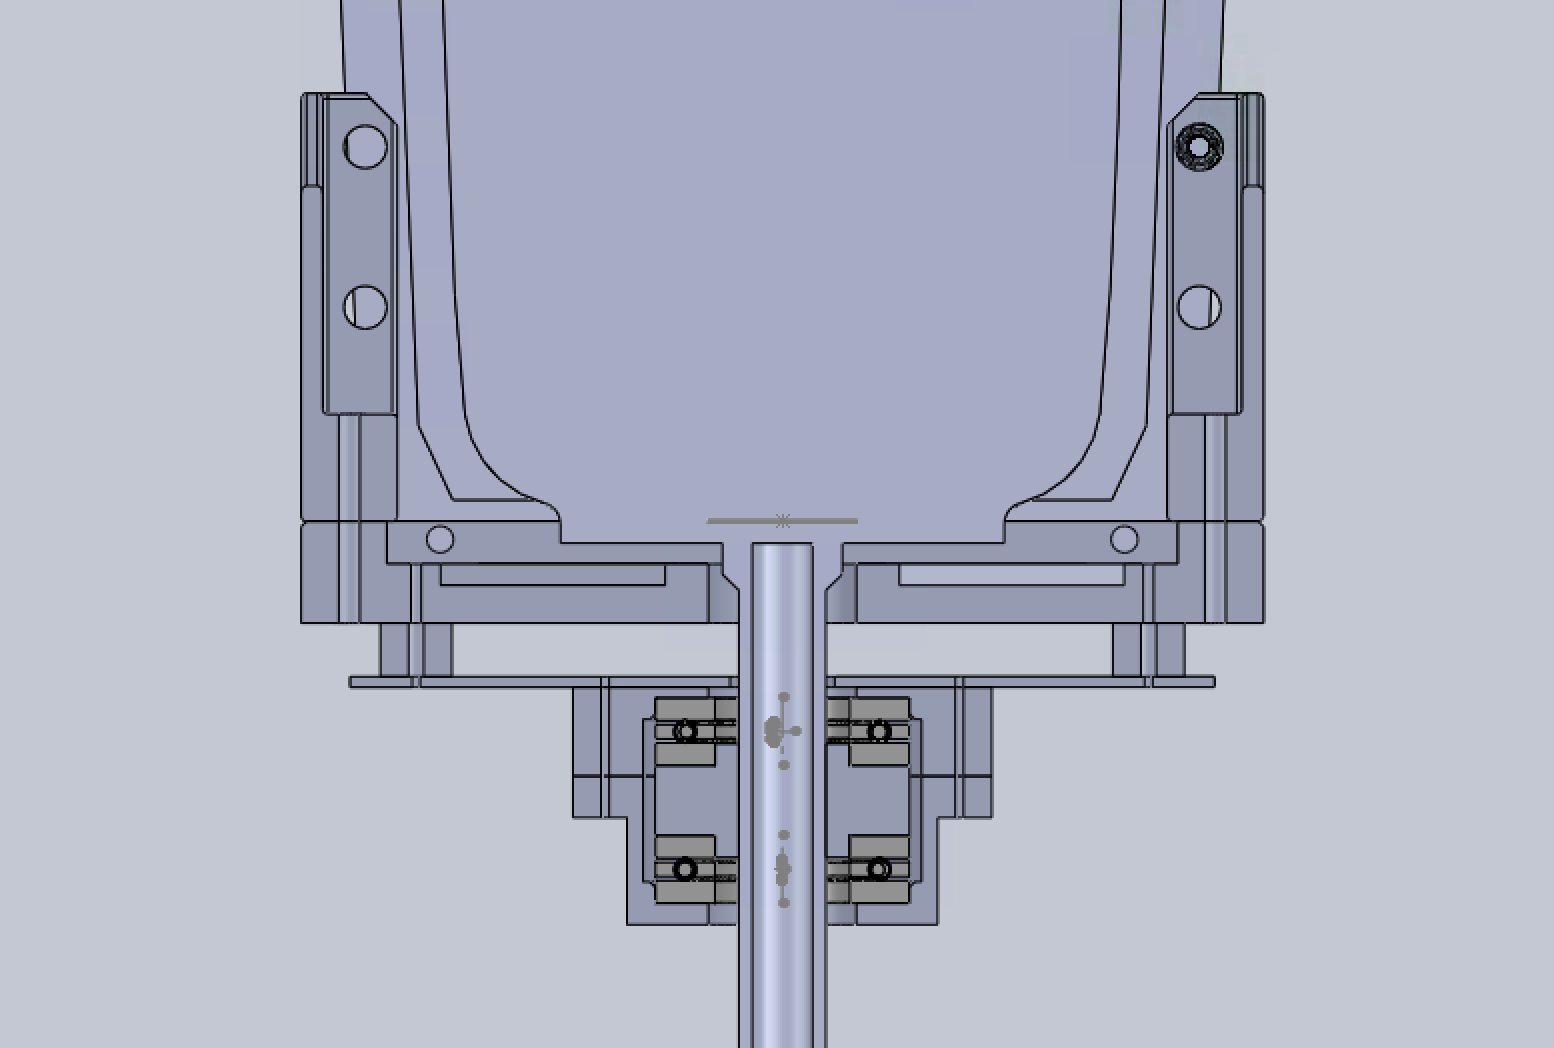
\includegraphics[width=80mm]{fig/methods/z_dir_sec.png}
	\end{center}
	\vspace{-4mm}
	\caption[Z-direction force feedback sensor - section vew]
	{Z-direction Force Feedback Sensor (Section View)}
	\label{fig:Z-direction_sec}
	\vspace{-2mm}
\end{figure}


Z-device (Figures \ref{fig:Z-direction}, \ref{fig:Z-direction_sec}) consists of attachment to the sterile adapter, 2 thrust ball bearings, three rings, plate, and two cylindrical spacers. Three rings and two ball bearings are used to transfer only z-directional forces further to the plate and keep ability of the shaft to rotate. The ring in the center is in direct contact with the instrument shaft, two outer rings are for the push and pull forces transfer. The plate experience maximum strain and all strain gauge sensors are mounted on it.  Two cylindrical spacers are used to give plate space to move and they are mounted on the attachment plate. the attachment plate consist of three plates, they are press fitted on the sterile adapter and fixed with four set screws.

Three rings and plate were manufactured with Aluminum Alloy 6061, attachment parts were 3-D printed, fasteners were used as spacers.


\section{Electrical and Software Design}
\label{sec:elecDes}

	\subsection{Circuit design}
	\label{sec:cirDes}
	Block diagram of the developed PCB is shown on Figure \ref{fig:PCB_block_diag}. Signal waveforms are shown on Figure \ref{fig:Wave_Out}.

\begin{figure}[h]
	\begin{center}
		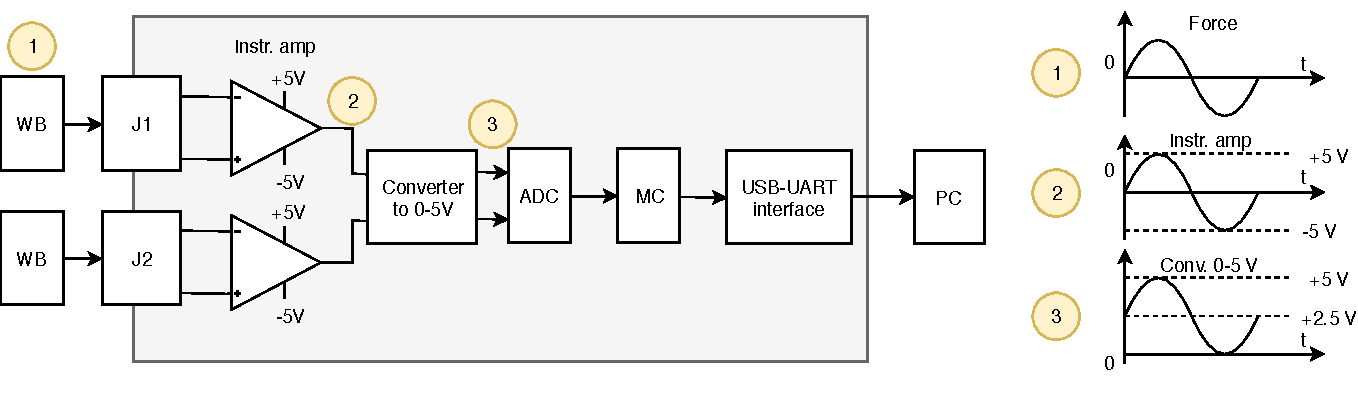
\includegraphics[width=150mm]{fig/methods/PSC_block_wave.pdf}
	\end{center}
	\vspace{-4mm}
	\caption[Block diagram of the circuit]
	{Block Diagram of the Circuit}
	\label{fig:PCB_block_diag}
	\vspace{-2mm}
\end{figure}
%\begin{figure}[h]
%	\begin{center}
%		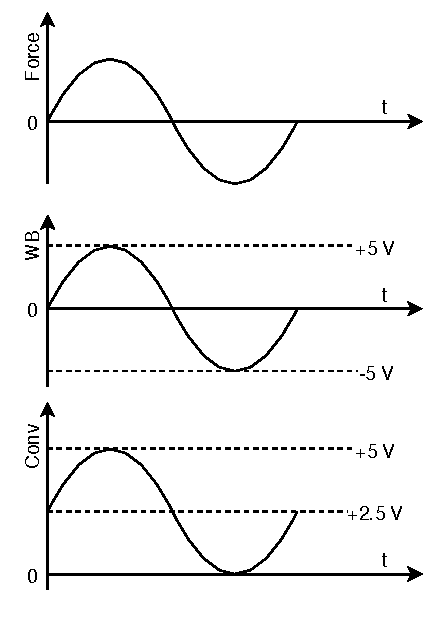
\includegraphics[width=60mm]{fig/methods/signal_diag.pdf}
%	\end{center}
%	\vspace{-4mm}
%	\caption[Signal Waveforms]
%	{Signal Waveforms}
%	\label{fig:Wave_Out}
%	\vspace{-2mm}
%\end{figure}

Four strain gauges are connected to form a wheatstone bridge circuit. On Figures \ref{fig:WB_xy_dev} - \ref{fig:WB_z} placement of strain gauges (1-4) and their wheatstone bridge configurations are shown for both devices. Strain gauges deform due to applied forces, and it causes voltage change on wheatstone bridge. Output signal from the wheatstone bridge goes to the instrumentation amplifier. Since ADC can convert only positive voltage, voltage converter changes voltage range of the output signal from ($-5V$ to $+5V$) to ($0V$ to $+5V$) range. That signal is converted to digital signal with 16-bit ADC, which communicates with the microcontroller via SPI interface. The output signal is transferred to the computer via USB. 
	
\begin{figure}[h]
	\begin{center}
		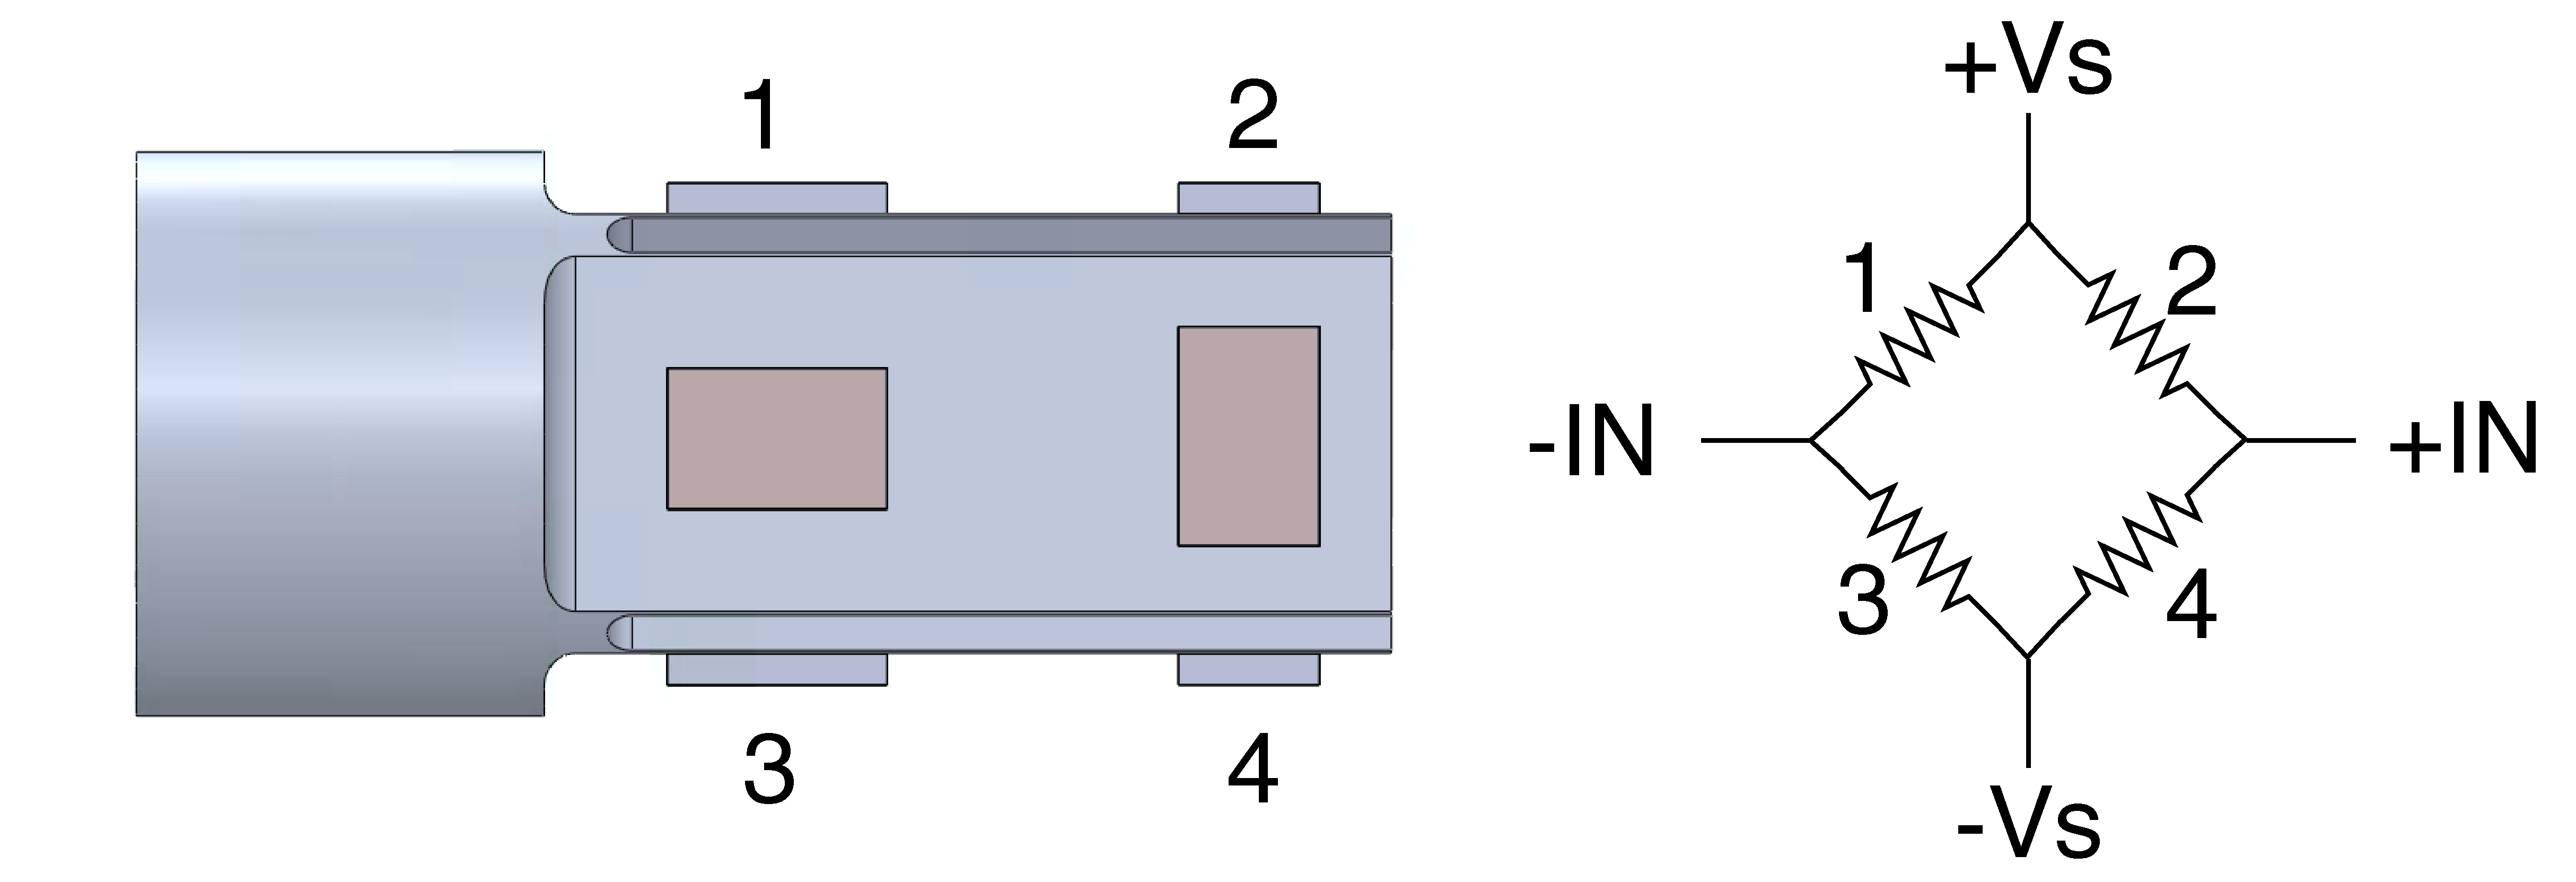
\includegraphics[width=120mm]{fig/methods/Wiring_xy_sleeve.pdf}
	\end{center}
	\vspace{-4mm}
	\caption[Wheatstone bridge configuration of XY-device]
	{Wheatstone Bridge Configuration of the XY-device}
	\label{fig:WB_xy_dev}
	\vspace{-2mm}
\end{figure}

\begin{figure}[h]
	\begin{center}
		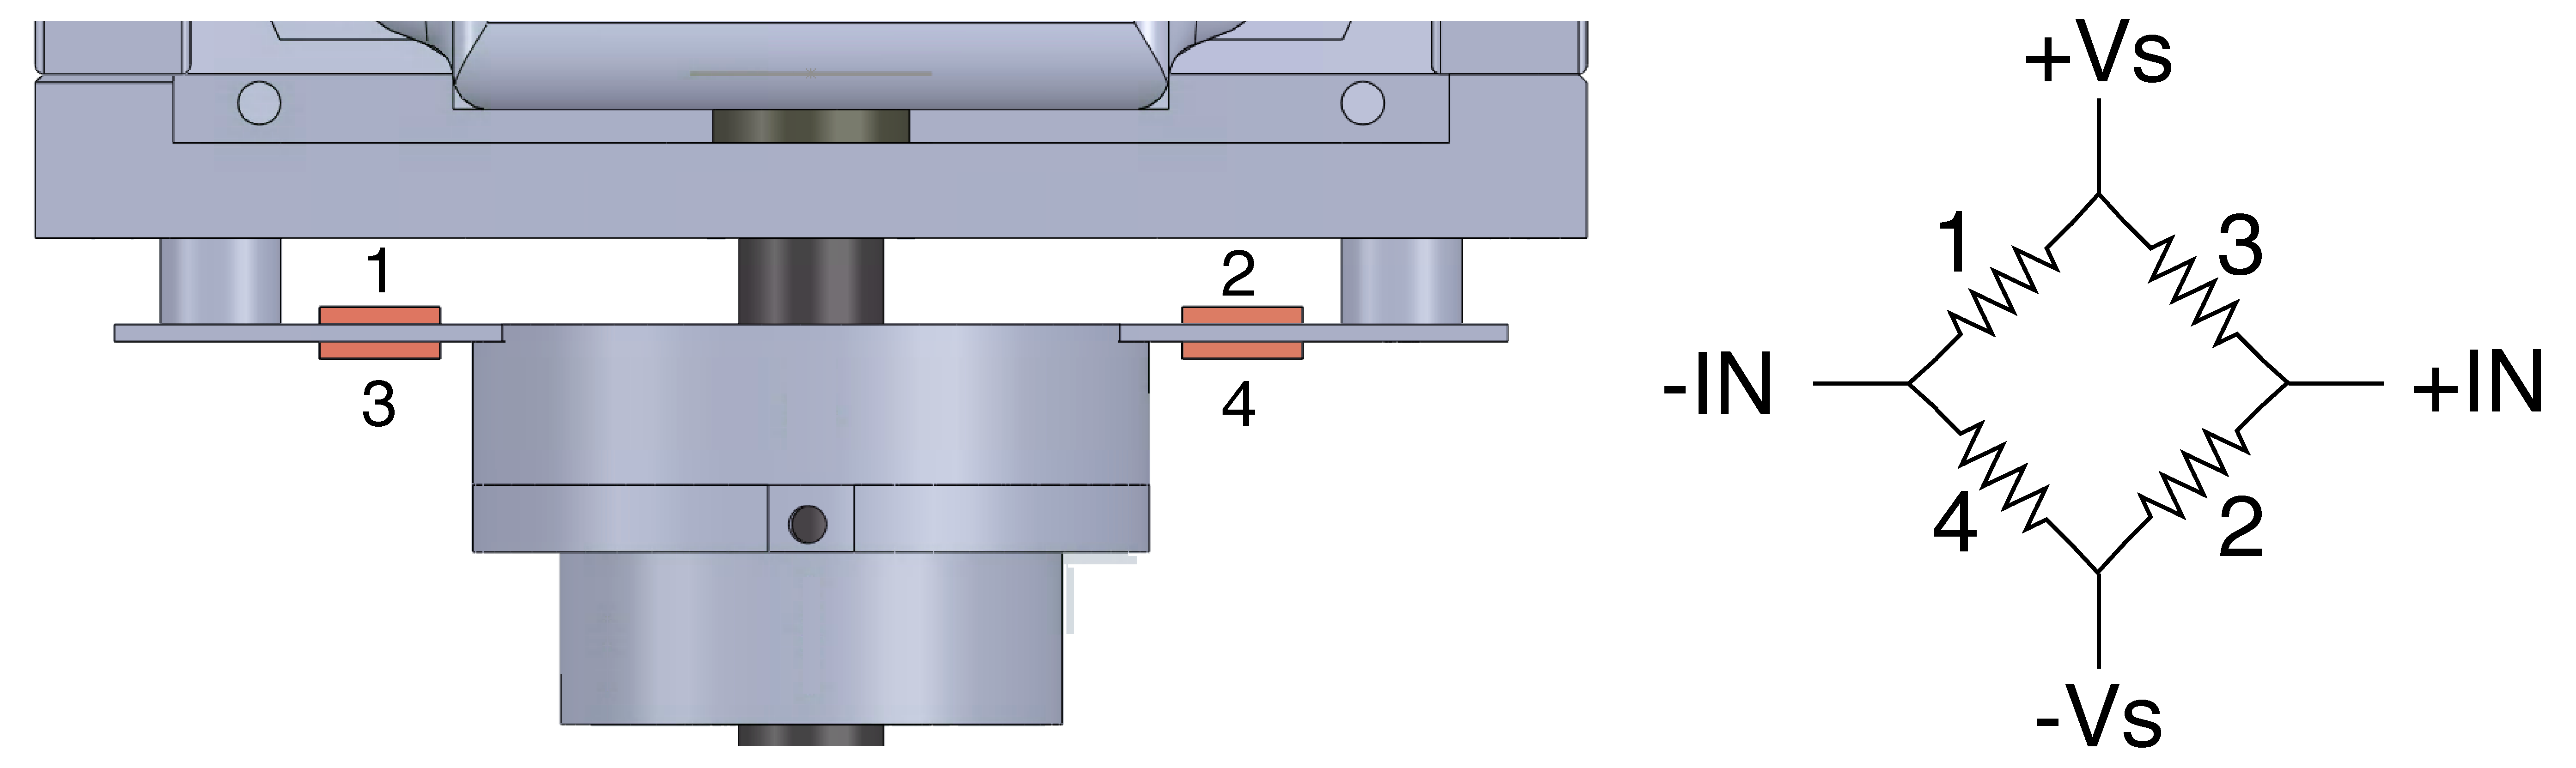
\includegraphics[width=140mm]{fig/methods/Wiring_z.pdf}
	\end{center}
	\vspace{-4mm}
	\caption[Wheatstone bridge configuration of Z-device]
	{Wheatstone Bridge Configuration of the Z-device}
	\label{fig:WB_z}
	\vspace{-2mm}
\end{figure}
	
\begin{figure}[h]
	\begin{center}
		\includegraphics[width=120mm]{fig/methods/PCB_real_look.png}
	\end{center}
	\vspace{-4mm}
	\caption[Manufactured PCB]
	{Manufactured PCB}
	\label{fig:PCB_real}
	\vspace{-2mm}
\end{figure}
	
Using Altium Designer 15.1 the PCB design was developed and manufactured at Advanced Circuits \cite{PCB_manufacturer}. 

In the developed PCB (Figure \ref{fig:PCB_real}) trimpots are used for calibration of the instrumentation amplifier gain (shown yellow) and change of reference voltage (shown red).

Instrumentation amplifier gain change is needed to set up appropriate measuring force range (0-11 N). During calibration, when 11 N applied on the tool end, the output signal (that goes to ADC) should be smaller than 4.5 V. When the same force applied in the opposite direction, the output signal should be bigger than 0.5 V.
 
Reference voltage change is used for the compensation of wheatstone bridge unbalance caused by strain gauge resistance tolerances. During the calibration, it should be tuned until it gives the output signal close to 2.5 V, when no forces applied on the device.

More details on the developed PCB are on github link.

	\subsection{Noise Analysis}
	\label{sec:NoiseExp}
	Fast Fourier transform (FFT) waveform analysis of the noise signal was performed using Tektronix MSO 4034 Mixed Signal Oscilloscope. The oscilloscope automatically applied the Hanning window, which has good frequency resolution and reduced spectral leakage\cite{harris_use_1978}.
	
\begin{figure}[h]%
\centering
\subfigure[1st Channel]{%
\label{fig:first}%
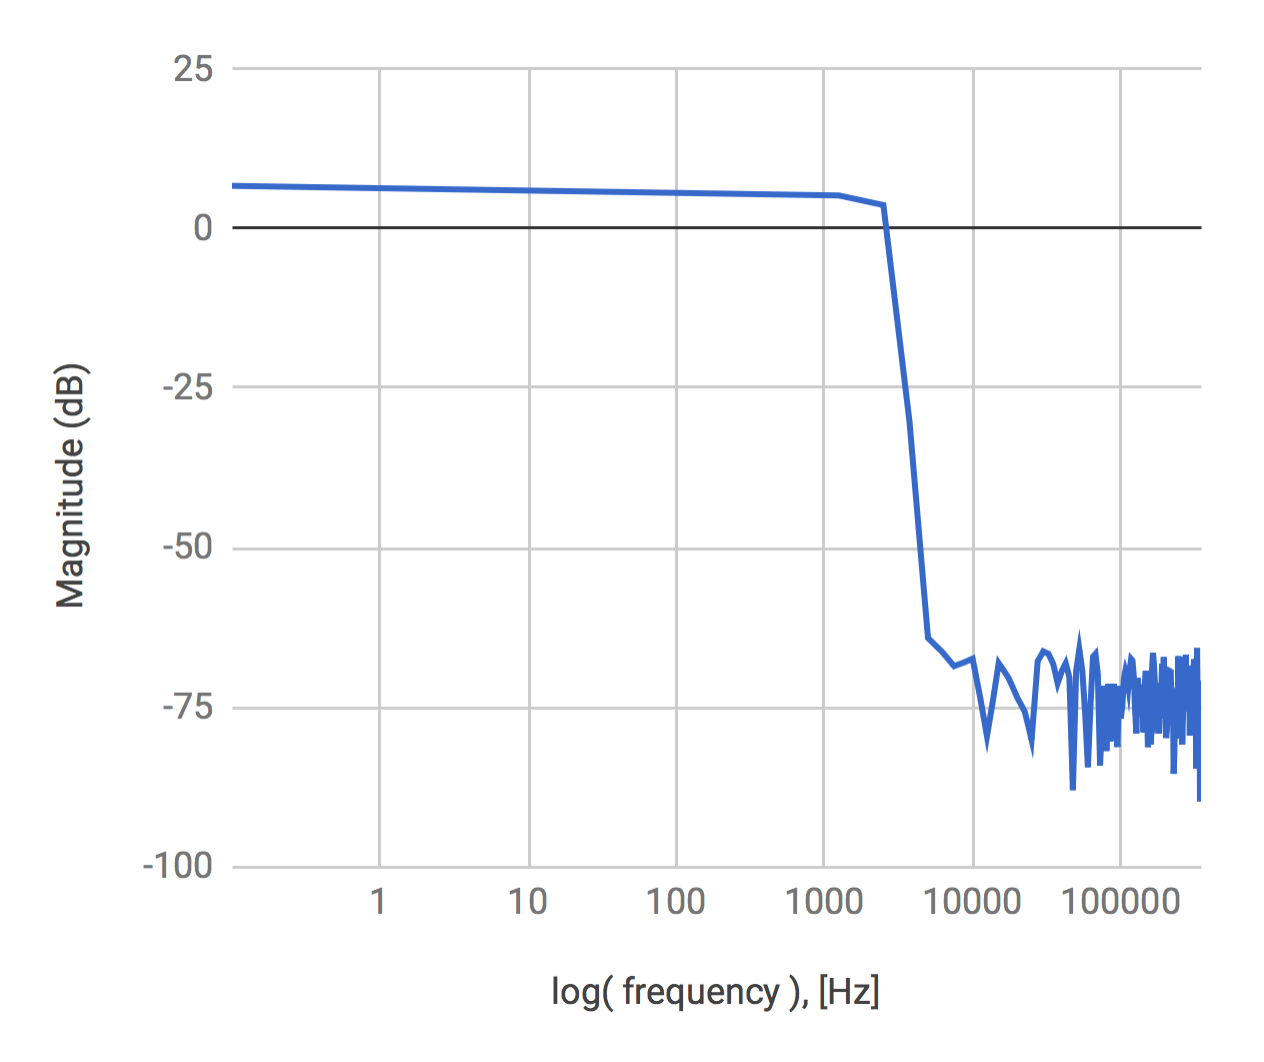
\includegraphics[height=2.2in]{fig/methods/noise_1_log.png}}%
\qquad
\subfigure[2nd Channel]{%
\label{fig:second}%
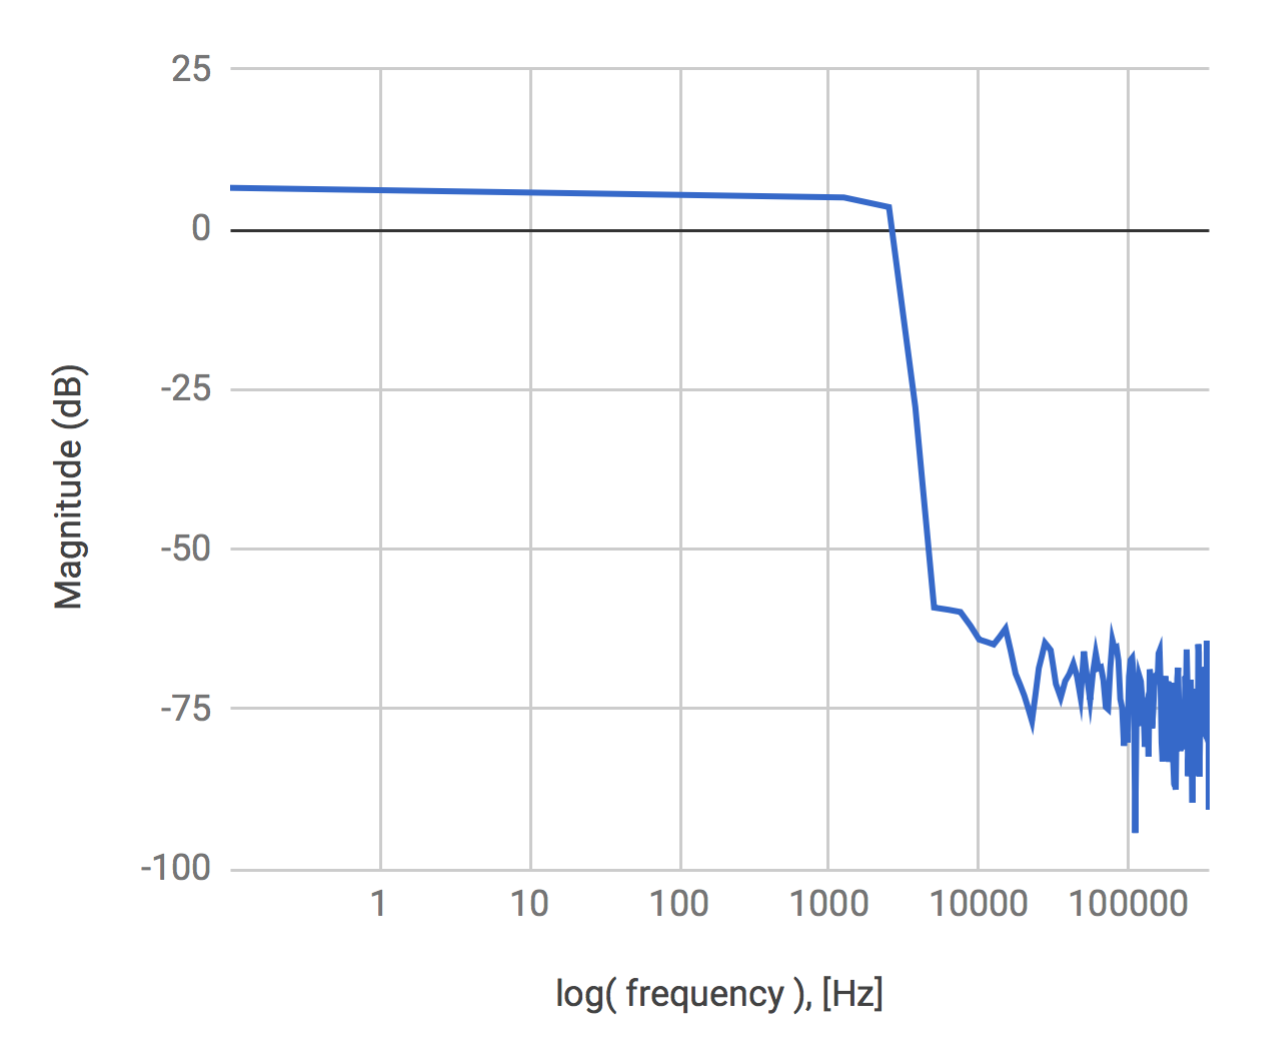
\includegraphics[height=2.2in]{fig/methods/noise_2_log.png}}%
\caption{FFT Analysis Results}
\end{figure}
	
	The signal frequency from the force sensor should be in range of (0 to 1 kHz). From the FFT analysis it can be concluded, that the noise frequency is in range (2.5 kHz and higher) with amplitude (-50 mV to 70 mV) for both channels. That means, low pass filter with cutoff frequency 2 kHz should be applied on the output signal. It was decided to use data averaging due to its simplicity of implementation and small time delays. It is an equivalent of low pass filtering that compensates the high frequency noise \cite{filtering_mov_ave}.

	\subsection{Microcontroller Software}
	\label{sec:MicrSoft}
	Microcontroller ATMEGA328P is used in the developed PCB for acqusition, filtering, and sending data to ROS. Main advantage of this microcontroller is that it has open-source packages for serial communication with ROS. The microcontroller is programmed to initialize ros nodes with names "adc\textunderscore xy" for XY-device and "adc\textunderscore zlc" for Z-device. The master-slave communication is created between X-Y and Z- devices for data acquizition synchronization by sending start conversion signals between two PCBs. When one of the devices gets the signal it starts to communicate with ADC though SPI interface (Figure \ref{fig:SPI_com}) \cite{introduction_SPI}. The acquired data is filtered from the high frequency noise by averaging of the 5 most recent readings. And the filtered data is published through the serial port with the baud rate 115200 bits per second. 
	
\begin{figure}[h]
	\begin{center}
		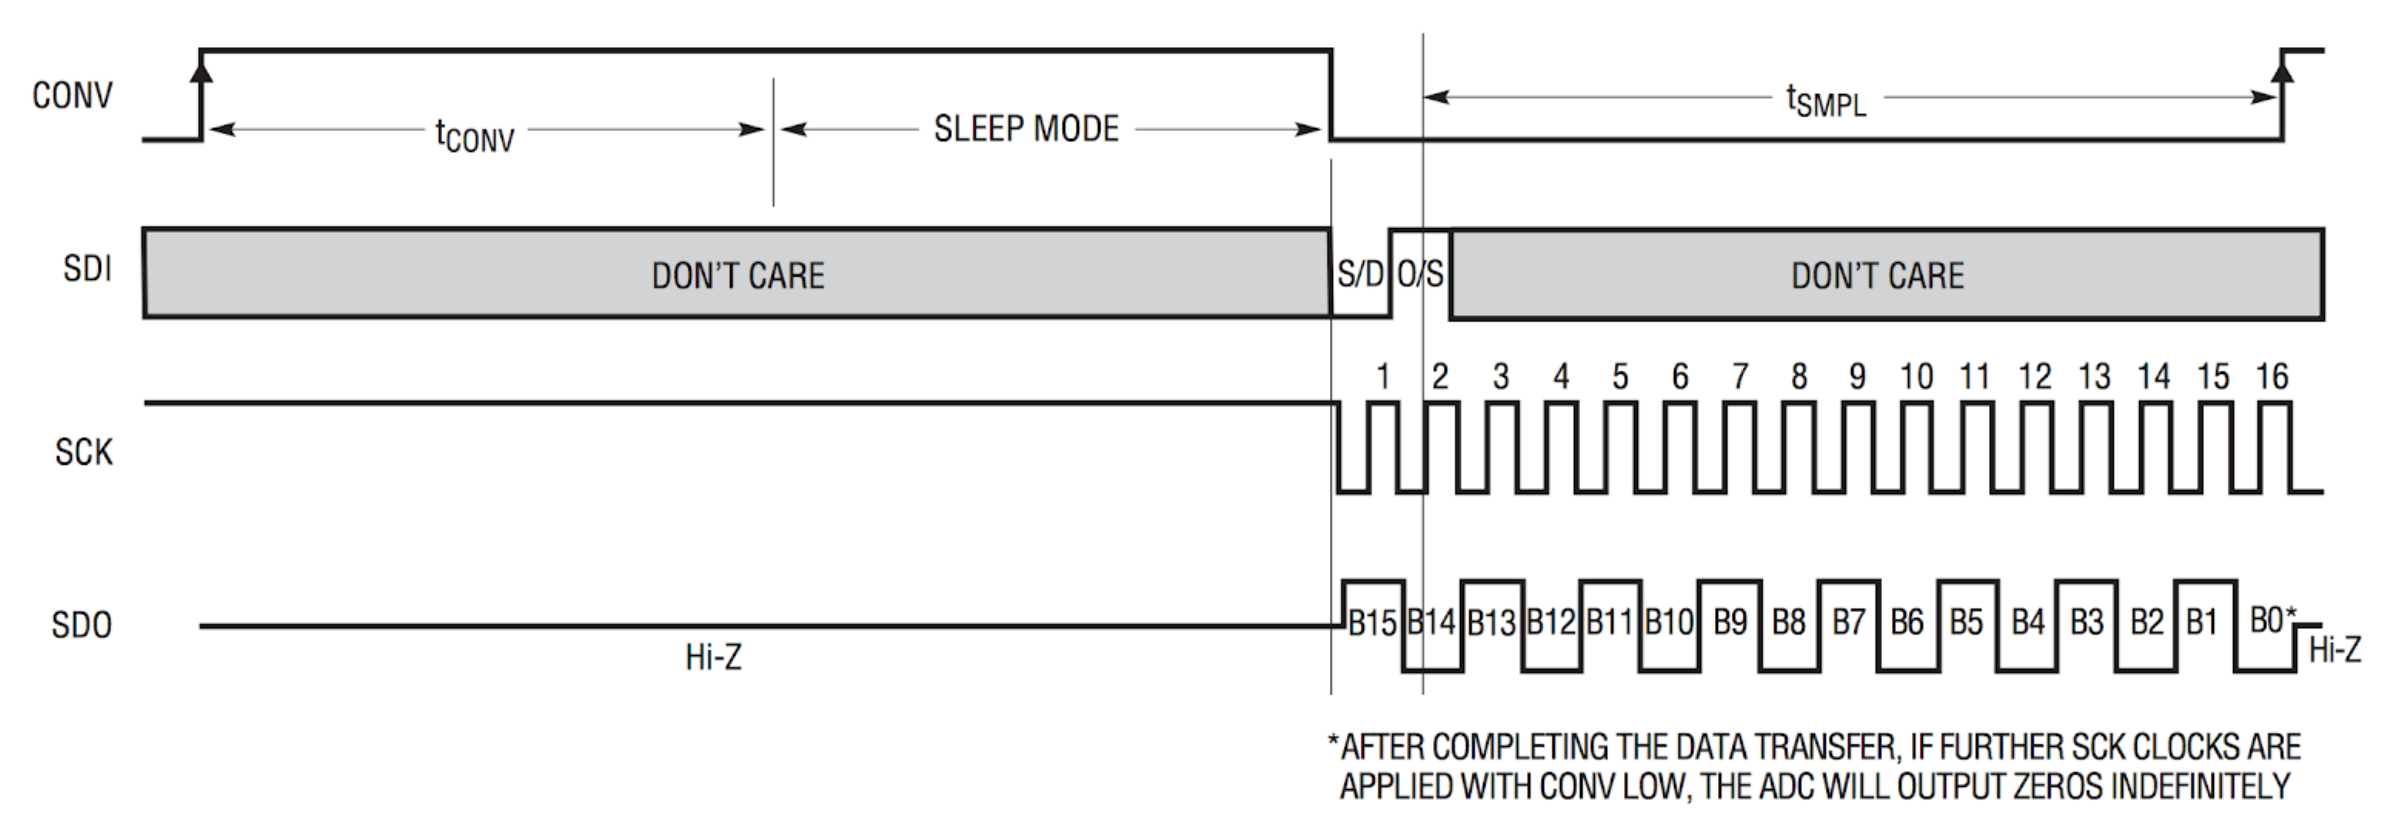
\includegraphics[width=140mm]{fig/methods/SPI_communication.png}
	\end{center}
	\vspace{-4mm}
	\caption[ADC LTC1865 Operating Sequence]
	{LTC1865 Operating Sequence \cite{ltc1865}}
	\label{fig:SPI_com}
	\vspace{-2mm}
\end{figure}

The github link to master device code and slave-device code.

	\subsection{ROS Architecture}
	\label{sec:p2}
Figure \ref{fig:ROS_arch} shows the ROS architecture of the developed system. In the python script we create a \textit{force\textunderscore feedback} node. The node is subscribed to X, Y, Z ADC data acquired form sensors and position of the sterile adapter from the daVinci controller. These data are used to find forces. The calculated forces (\textit{force\textunderscore x, force\textunderscore y, force\textunderscore z}) are then published.
\begin{figure}[h]
	\begin{center}
		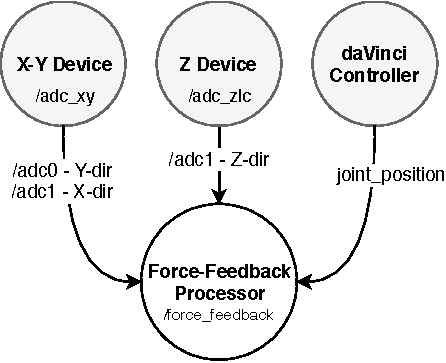
\includegraphics[width=80mm]{fig/methods/ROS_architecture.pdf}
	\end{center}
	\vspace{-4mm}
	\caption[ROS architecture]
	{ROS Architecture}
	\label{fig:ROS_arch}
	\vspace{-2mm}
\end{figure}	

The program calculates magnitude of the forces in X, Y, Z directions using the calibration equation:
\begin{equation}\label{eq:calib_eq}
F = \frac{adc_{data} - b}{a}
\end{equation}

where $b$ is the constant equal to ADC reading when $F = 0$, $adc_{data}$ is current sensor reading in corresponding direction, and $a$ is linear function of sterile adapter position:
\begin{equation}\label{eq:ster_adap_pos}
a = c \cdot position + d
\end{equation}

where $c$ and $d$ are constants found during calibration and $position$ is the position of the sterile adapter.
 
	%To make communication between microcontroller and ROS work it is necessary to install rosserial\textunderscore arduino package \cite{rosserial_arduino}.
	
\section{Calibration}
\label{section:Calibration}

	\subsection{Calibration Setup}
	\label{sec:CalSetup}
	In order to find parameters of the calibration equation (\ref{eq:calib_eq}), the calibration system was developed (Figure \ref{fig:Calib_setup_BD}). Load cell and Polaris optical tracking system are used to find "true" force applied to the tool end. The load cell is used to find the magnitude of the applied force and the optical trackers (4-5) to find the direction of the force.
	
	During the calibration user should first calibrate the load cell. Then insert the tool in the sterile adapter.  The force readings depend on the position of the sterile adapter, meaning that the force/sensor readings curve should be found for different positions of the adapter. Finding the curve for only two positions would be enough, because the correlation between the curve and position is linear, as equation (\ref{eq:ster_adap_pos}) shows. 
	
\begin{figure}[h]
	\begin{center}
	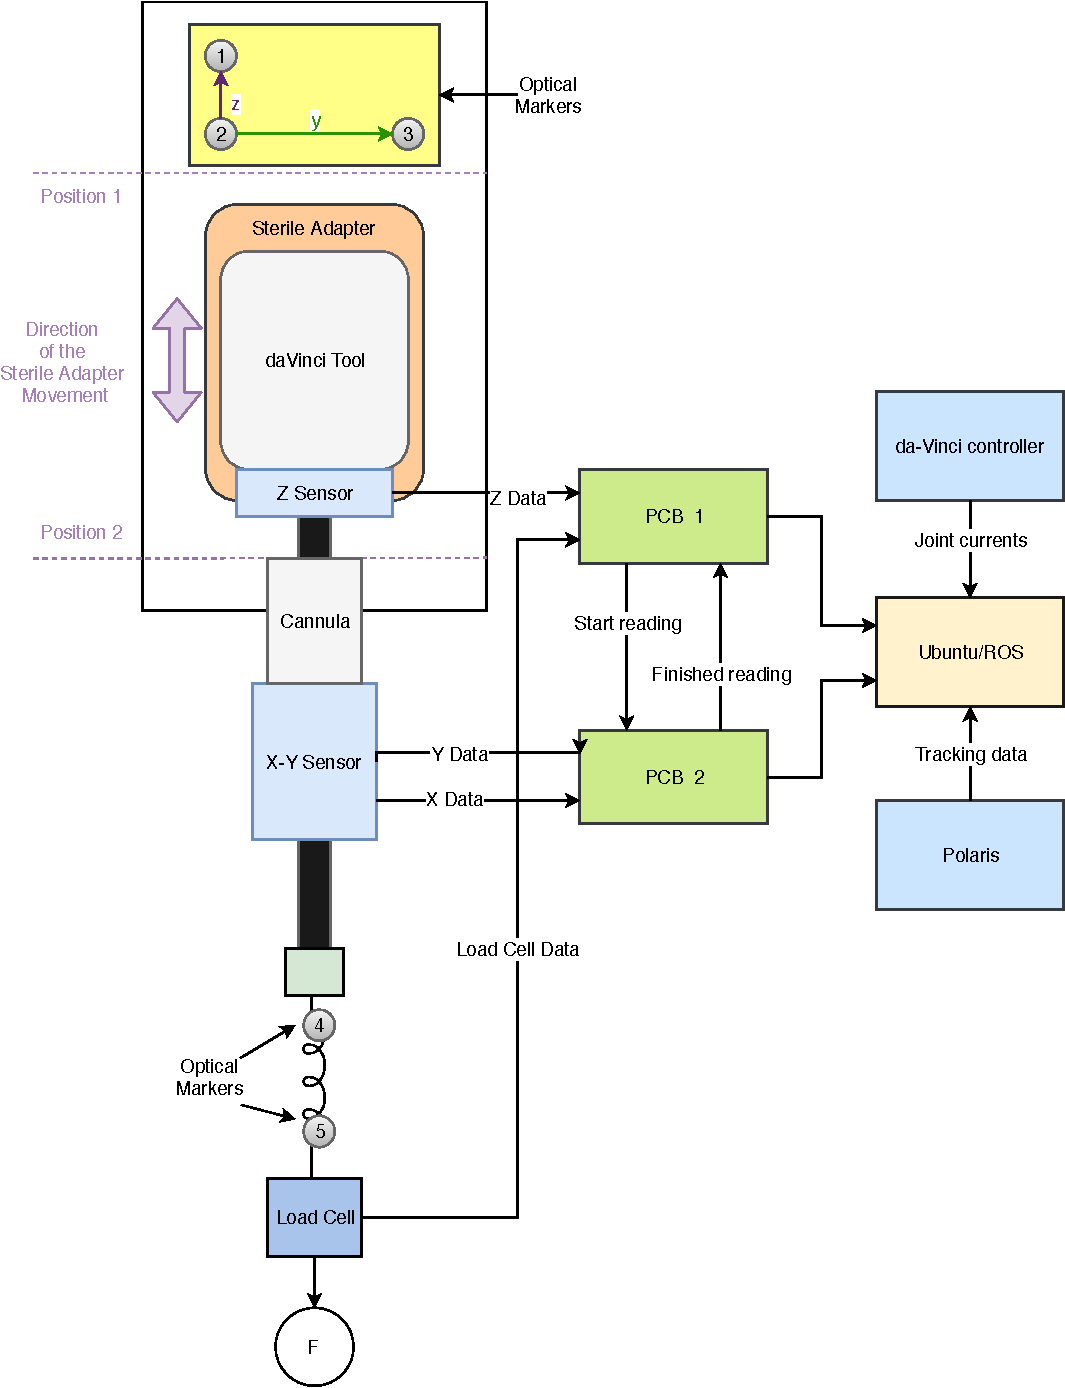
\includegraphics[width=100mm]{fig/methods/block_diagram_of_calib_setup.pdf}
	\end{center}
	\vspace{-4mm}
	\caption[Block Diagram of the Calibration Setup]
	{Block Diagram of the Calibration Setup}
	\label{fig:Calib_setup_BD}
	\vspace{-2mm}
\end{figure}

Before starting data collection, the PSM joint of the sterile adapter should be fixed in position 1. After fixing the adapter, in order to transform Polaris camera frame to the robot frame, the transformation matrix should be found. For this purpose, three optical markers (1-3) are attached to the PSM. Z-direction vector corresponds to the vector formed by (2-1) optical markers, Y-direction vector is formed by (2-3) optical markers. X-direction vector can be found as a cross product between these two vectors:
\begin{equation}
\vec{X} = \vec{Y}\times \vec{Z}
\end{equation}
Using found $\vec{X}$, $\vec{Y}$, $\vec{Z}$ vectors and taking the position of (2) optical marker as a position of the origin vector. The transformation matrix can be found:
\begin{equation}
T_{w}^{c} = 
\begin{bmatrix}
    X_{x} 	& Y_{x} 		& Z_{x} 		&  x_{0} \\
    X_{y} 	& Y_{y} 		& Z_{y} 		&  y_{0} \\
    X_{z} 	& Y_{z} 		& Z_{z} 		&  z_{0} \\
    0		 	& 0 			& 0 			& 1
\end{bmatrix}
\end{equation}


	\subsection{Calibration of the Load Cell}
	\label{sec:CalLoadCell}
	Was performed using following setup cite figure ..
	Calibration equation we got ..

	\subsection{Calibration Results}
	Find mean square root error

		\begin{figure}
			\centering
			\begin{subfigure}
				\centering
				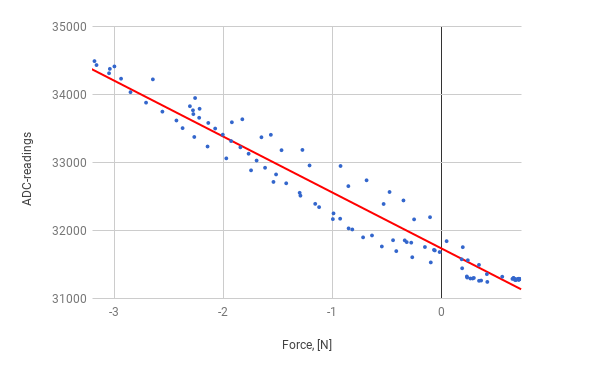
\includegraphics[width=120mm]{fig/results/x-dir.png}
				\caption{X-component}
				\label{fig:Xdirection}
			\end{subfigure}
			\begin{subfigure}
				\centering
				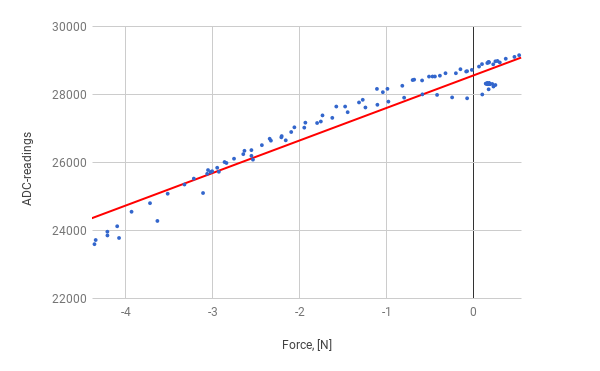
\includegraphics[width=120mm]{fig/results/y-dir.png}
				\caption{Y-component}
				\label{fig:Ydirection}
			\end{subfigure}
			\caption{Calibration results}
			\label{fig:Calibration}
		\end{figure}
Precision represents capacity of a sensing system to give the same reading when repetitively measuring the same measurand under the same conditions. The precision is a statistical parameter and can be assessed by the standard deviation (or variance) of a set of readings of the system for similar inputs.

One of the measurements of signal quality is signal-to-noise ratio (SNR). A higher value of SNR means the clear acquisitions with low signal distortions and artifacts caused by unwanted noise. It is defined as:

\begin{equation}
\frac{S}{N}=\frac{Mean value of signal}{Standard deviation of noise}
\end{equation}

For X-direction SNR is $3232 \pm 78$, for Y-direction SNR is $2857 \pm 150$, which is much bigger than 1. It means that system has very low noise.

Error is the difference between the actual value of the measurand and the value produced by the sensing system. Error can be caused by a variety of internal and external sources and is closely related to accuracy. Accuracy can be related to absolute or relative error as:

\begin{equation}
Absolute error = \frac{Output}{ True value}
\end{equation}

From figure we can assume that fluctuations in the output signal are due to systematic errors. 

Drift is observed when a gradual change in the sensing system’s output is seen, while the measurand actually remains constant. Drift is the undesired change that is unrelated to the measurand. It is considered a systematic error, which can be attributed to interfering parameters such as mechanical instability and temperature instability, contamination, and the sensor’s materials degradation. 

Resolution (or discrimination) is the minimal change of the measurand that can produce a detectable increment in the output signal. Resolution is strongly limited by any noise in the signal.

In a sensing system, minimum detectable signal (MDS) is the minimum signal increment that can be observed, when all interfering factors are taken into account. When the increment is assessed from zero, the value is generally referred to as threshold or detection limit. If the interferences are large relative to the input, it will be difficult to extract a clear signal and a small MDS cannot be obtained.

Sensitivity is the ratio of the incremental change in the sensor’s output (Dy) to the incremental change of the measurand in input (Dx). The slope of the calibration curve, y f(x), can be used for the calculation of sensitivity.

The closeness of the calibration curve to a specified straight line shows the linearity of a sensor. Its degree of resemblance to a straight line describes how linear a system is.

Hysteresis is the difference between output readings for the same measurand, depending on the trajectory followed by the sensor.

The maximum and minimum values of the measurand that can be measured with a sensing system are called the measurement range, which is also called the dynamic range or span. This range results in a meaningful and accurate output for the sensing system. \cite{kalantar-zadeh_sensors_2013}

\section{Experiments}
\label{sec:Experims}

	\subsection{Distance from the cannula to the tip dependence from readings}
	\label{sec:DisExp}
	Distance from the cannula to the tip - measure - 3 ¼ inch. Maximum distance is 9 inches.


	\subsection{Temperature Dependence}
	\label{sec:TempExp}
	Try in 36.6 Celsius and room temperature
	Effect of the surrounding temperature on the device was ..

	Do all experiments at least three times and calculate all statistic things you can (SD)

	\subsection{Hysteresis}
	\label{sec:HystExp}
	Hysteresis was checked .. 
	We written separate program to check hysteresis






\chapter{Discussion and Conclusion}
\label{discuss} % Always give a unique label

Some of the requirements for the device were satisfied. However, some of the major ones were not, meaning that the devices need further improvements.
	
	Both devices should undergo sterilization. One of the devices goes inside the patient, meaning that it should be created using biocompatible materials. Current version of the device is not biocompatible. We can achieve biocompatibilty by using Stainless Steel as a device material and biocompatible epoxy to cover strain gauges, also teflon coated wires should be used for all electrical connections. Use of stainless steel will require change of the device dimensions, since the material has different elasticity. Also, epoxy cover can alter readings results.
	
	The real-time haptic feedback requires minimum data acquisition speed to be 1 kHz \cite{seungmoon_choi_effect_2004}. However, the current maximum speed is 588 Hz due to limitation of data transfers speed using serial communication with computer (115.2 Kbps). In order to increase the speed, we can change the communication channel to SPI (up to 10 Mbps) \cite{_uart_porotocol} or one of the wireless protocols, such as Bluetooth (up tp 1 Mbps) or wifi (up to 100 Mbps) \cite{_wireless_protocols}. Also, communication protocol between microcontroller and ADC can be changed from SPI to faster parallel communication. Additionally, the microcontroller can be changed to faster one, so it can support wireless communication.
	All these changes require change of PCB design and microcontroller software. Also, in the PCB the amount of Wheatstone bridges and ADCs should be increased from 2 to 4 to decrease the overall size of the system by removing second PCB and master-slave communication.
	
	The designed devices measure forces in slightly higher than $\pm 11 N$ range. When the applied force exceeds the specified range, the device redaings can be used to trigger safety alert.
	
	The required resolution should be at least 0.3 N and have error less than 0.05 N \cite{mack_interactive_2012}.
	

We can use QTC-pills in future, promising approach, higher sensitivity 
	
	 The system has separate wheatstone bridges for each direction, giving ability to measure each component of the force independently. At the same time tool can rotate freely and changing the insertion depth.	
	
	Strain gauges have linear response with deformation. Our calibration results have shown linearity of the readings.

	Force-sensing devices were designed to fit daVinci cannula and sterile adapter and compensate tolerances by adjustment of set screws.

SNR values for all systems are bigger than 1, meaning that all systems have relatively low noise.

Figure \ref{fig:Syst_err} shows X-component of the force measured with created device and using load cell. SNR of the system is high  it can be assumed that fluctuations in the output signal are due to systematic errors. 

For Z-direction device we got wide range of forces, because we cannot get high electronic gain, since the sensor is unbalanced caused by mechanical preloading of the sensor plate.

Temperature dependence is not appropriate to do, since we have big systematic errors. First priority will be remove systematic errors.

\begin{figure}[h]
	\begin{center}
	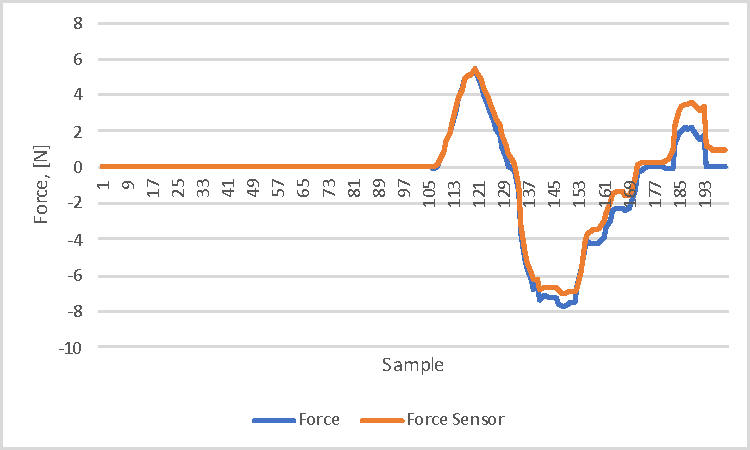
\includegraphics[width=80mm]{fig/results/syst_error.pdf}
	\end{center}
	\vspace{-4mm}
	\caption[Actual and Measured Forces in X-direction]
	{Actual and Measured Forces in X-direction}
	\label{fig:Syst_err}
	\vspace{-2mm}
\end{figure}

This is our conclusion)

For future work ..
However, disadvantages would be addition of the cost to already expensive system and possible biocompaitibily and sterilization issues. Also addition of the weight to the arm could alter robot performance, however, since the device will be placed close to center of rotation of the robot arm, it will have minimal affect on the moment of inertia  in comparison to sensors added to the grippers.


\begin{figure}[h]
	\begin{center}
		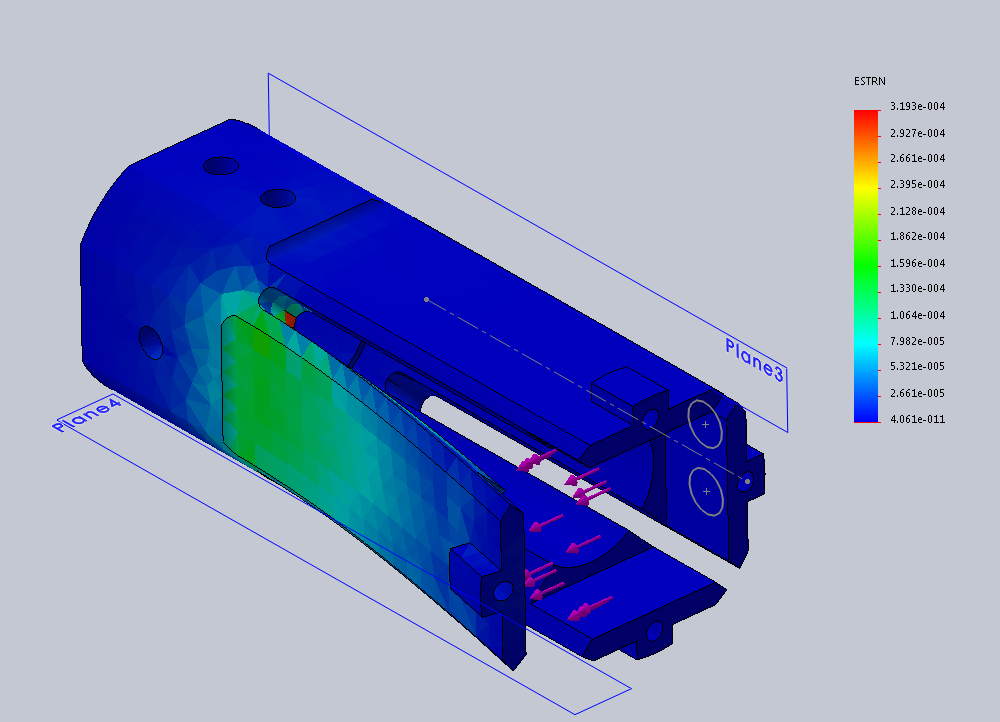
\includegraphics[width=120mm]{fig/methods/NEW_SLEEVE_STRAIN.png}
	\end{center}
	\vspace{-4mm}
	\caption[New X-Y Device Design]
	{New X-Y Device Design}
	\label{fig:NewXYDesign}
	\vspace{-2mm}
\end{figure}

Z-direction. We tried to measure force in Z-direction, but unfortunately results shown that developed system was not accurate and sensitive enough. To improve system we can suggest to change strain gauges to more sensitive ones. Since we have small room for deformation - around 0.3 mm, we can not afford more deformation by using thinner or longer plates. Therefore, we decided to use motor current readings for z-directional reading of the force.



%% REFERENCES
% if you use BIBTEX
\begin{spacing}{1}
\def\dsp{\def\baselinestretch{1.25}\large\normalsize}
\bibliographystyle{template/IEEEtran}
\bibliography{bibliography}
\end{spacing}
\end{document}
